%% ---------------------------------------------------------------------------
%%  Pencarian Terpadu Tahan Salah Ketik pada OpenMRS
%%  Format: IEEE Transactions (ieeecolor.cls), susunan bab IMRAD
%%  Kompilasi:  pdflatex main -> pdflatex main   (bibliografi manual, tanpa BibTeX)
%%  Seluruh angka pada berkas ini bersumber dari riset/hasil4..hasil6 di repo yang
%%  sama; gambar dibangun ulang oleh gambar/buat_gambar.py langsung dari JSON hasil.
%% ---------------------------------------------------------------------------
\documentclass[journal,twoside,web]{ieeecolor}
\usepackage{generic}
\usepackage[T1]{fontenc}
\usepackage[utf8]{inputenc}
\usepackage{cite}
\usepackage{amsmath,amssymb,amsfonts}
\usepackage{algorithmic}
\usepackage{graphicx}
\usepackage{algorithm,algorithmic}
\usepackage{booktabs}
\usepackage{multirow}
\usepackage{longtable}
\usepackage{url}
\usepackage{hyperref}
\hypersetup{hidelinks=true}
\usepackage{textcomp}
\usepackage[english,indonesian]{babel}   % pola pemenggalan suku kata bahasa Indonesia

\graphicspath{{gambar/}}

% -- Label abstrak dapat diganti, supaya abstrak Indonesia dan Inggris
%    memakai judulnya masing-masing. Salinan definisi ieeecolor.cls dengan
%    kata "Abstract" digantikan makro \abslabel.
\makeatletter
\newcommand{\abslabel}{Abstract}
\def\abstract{\everymath={\sf}\sf%
    \if@twocolumn%
      \if@web  \definecolor{nblue}{rgb}{0,0.263,0.576}%
        \definecolor{mblue}{rgb}{0.075,0.541,0.855}%
      \else
        \definecolor{nblue}{cmyk}{0,0,0,1}%
        \definecolor{mblue}{cmyk}{0,0,0,1}\fi
      \if@shortpaper
        \footnotesize\bfseries\color{subsectioncolor}\textit{\abslabel}---\,\normalcolor%
      \else
        \@IEEEabskeysecsize\bfseries\color{subsectioncolor}\textit{\abslabel}---\,\normalcolor%
      \fi
    \else%
      \begin{center}\vspace{-1.78ex}\@IEEEabskeysecsize\textbf{\abslabel}\end{center}%
      \quotation\@IEEEabskeysecsize%
    \fi\@IEEEgobbleleadPARNLSP}

% -- Label kata kunci, disesuaikan ke bahasa Indonesia dengan cara yang sama.
\newcommand{\keylabel}{Kata Kunci}
\def\keywords{\everymath={\sf}\sf%
    \if@twocolumn%
      \if@web  \definecolor{nblue}{rgb}{0,0.263,0.576}%
        \definecolor{mblue}{rgb}{0.075,0.541,0.855}%
      \else
        \definecolor{nblue}{cmyk}{0,0,0,1}%
        \definecolor{mblue}{cmyk}{0,0,0,1}\fi
      \if@shortpaper
        \normalsize\bfseries\color{subsectioncolor}\textit{\keylabel}---\,\relax\normalcolor%
      \else
        \@IEEEabskeysecsize\bfseries\color{subsectioncolor}\textit{\keylabel}---\,\relax\normalcolor%
      \fi
    \else%
      \begin{center}\@IEEEabskeysecsize\bfseries \keylabel\end{center}%
      \quotation\@IEEEabskeysecsize%
    \fi\@IEEEgobbleleadPARNLSP}
\makeatother

\def\BibTeX{{\rm B\kern-.05em{\sc i\kern-.025em b}\kern-.08em
    T\kern-.1667em\lower.7ex\hbox{E}\kern-.125emX}}

\markboth{\hskip18pc NASKAH PRAPUBLIKASI}
{Chrismawan \MakeLowercase{\textit{dkk.}}: Pencarian Terpadu Tahan Salah Ketik pada OpenMRS}

\begin{document}

\title{Pencarian Terpadu Tahan Salah Ketik pada Rekam Medis Elektronik Sumber
Terbuka: TF--IDF Hibrida Kata--Karakter dengan Fusi Peringkat Berbobot pada
OpenMRS}

\author{%
\begin{tabular}{@{}l@{\hspace{2.2em}}l@{}}
Stephen Prasetya Chrismawan & 25/563032/PPA/07093 \\
M. Syarif Hidayatullah      & 25/567018/PPA/07143 \\
Sampurno Aji                & 25/568826/PPA/07155 \\
Reza Purwantara Firdaus     & 25/565168/PPA/07125 \\
\end{tabular}
\thanks{Naskah diserahkan 3 September 2026. Penelitian ini dilaksanakan tanpa
pendanaan eksternal. Seluruh perangkat lunak, data eksperimen, dan berkas hasil
mentah yang mendasari angka pada naskah ini tersedia pada repositori penelitian
yang sama dengan naskah ini.}
\thanks{S.~P. Chrismawan (NIM 25/563032/PPA/07093;
e-mail: stephenprasetyachrismawan27@gmail.com), M.~S. Hidayatullah
(NIM 25/567018/PPA/07143), S.~Aji (NIM 25/568826/PPA/07155), dan
R.~P. Firdaus (NIM 25/565168/PPA/07125) adalah mahasiswa Program Studi
Ilmu Komputer, Program Pascasarjana.}
\thanks{Kode implementasi modul OpenMRS berada pada
\texttt{backend/openmrs-module-tfidf-search/}; skrip eksperimen dan berkas hasil
mentah pada \texttt{riset/}.}}

\maketitle

% =============================================================================
%  ABSTRAK
% =============================================================================
\renewcommand{\abslabel}{Abstrak}
\begin{abstract}
\textbf{Latar belakang.} OpenMRS adalah rekam medis elektronik sumber terbuka
yang banyak dipakai di fasilitas kesehatan berdaya rendah. Kotak pencariannya
menjadi pintu masuk hampir seluruh alur kerja klinis, namun hanya entitas konsep
yang memiliki pencarian tahan salah ketik; tujuh entitas lain tidak memilikinya
sama sekali, dan tidak ada satu pun kotak pencarian yang menjangkau seluruhnya.
\textbf{Tujuan.} Merancang, mengimplementasikan, dan mengevaluasi mesin
pencarian terpadu lintas-entitas yang tahan salah ketik, cukup ringan untuk
dijalankan tanpa GPU, tanpa server indeks terpisah, dan tanpa sambungan
internet. \textbf{Metode.} Delapan tabel OpenMRS diproyeksikan ke satu bentuk
dokumen virtual, lalu diindeks dua kali: sebagai token kata dan sebagai kepingan
karakter empat-gram, keduanya dengan pembobotan TF--IDF skema \emph{ltc}. Skor
kedua jalur digabung pada tingkat entitas (bobot jalur kata 0,20), lalu peringkat
antar-entitas disatukan dengan \emph{Weighted Reciprocal Rank Fusion}. Sistem
diuji pada 360 kueri sintetis berlabel atas korpus 8.045 dokumen (35.914
\emph{surface form}) demo data resmi OpenMRS, dengan pemisahan ketat 100 kueri
pengembangan dan 260 kueri uji yang hanya dijalankan sekali. Signifikansi diukur
dengan \emph{paired bootstrap}. \textbf{Hasil.} Sistem usulan mencapai nDCG@10
0,670 terhadap 0,631 milik baseline pencocokan awalan --- selisih +0,039 yang
\textbf{tidak mencapai signifikansi} (p=0,079). Keunggulan yang bertahan berada
pada dimensi lain: kueri tanpa hasil turun dari 15,4\% menjadi \textbf{0,0\%},
R@10 naik dari 0,594 menjadi 0,743, dan MRR dari 0,725 menjadi 0,780. Ablasi
menempatkan seluruh perolehan itu pada satu komponen, kepingan karakter (E1 vs
B1 +0,114, p<0,001), sedangkan fusi peringkat berbobot tidak menyumbang nDCG
(--0,011, p=0,406). Analisis per entitas menjelaskan sebabnya: sistem usulan
unggul jelas pada entitas berciri kamus (konsep +0,171, obat +0,232) dan
\textbf{kalah} pada entitas instans per-pasien yang judulnya berulang lintas
baris (hasil laboratorium --0,180, pasien --0,242). Terhadap endpoint pencarian
konsep OpenMRS yang sesungguhnya, selisihnya +0,055 (p=0,269), juga tidak
signifikan. Implementasi Java mereproduksi angka Python (b0 dan e3 cocok persis),
membangun 17 indeks dalam 2,08~detik, dan melayani kueri pada p95 50~ms.
\textbf{Simpulan.} Kepingan karakter menghapus jalan buntu pencarian secara
meyakinkan, tetapi keunggulan nDCG@10-nya tidak bertahan begitu korpus diperluas
ke entitas instans per-pasien. Manfaat metode ini bergantung pada sifat entitas
yang diindeks, bukan berlaku merata --- temuan yang hanya terlihat karena korpus
evaluasi disamakan dengan korpus yang benar-benar dipasang.
\end{abstract}

\begin{IEEEkeywords}
Perolehan informasi, rekam medis elektronik, OpenMRS, TF--IDF, kepingan karakter
($n$-gram), fusi peringkat resiprokal, toleransi salah ketik, informatika
kesehatan sumber terbuka.
\end{IEEEkeywords}

% =============================================================================
\section{Introduction}
% =============================================================================

\IEEEPARstart{R}{ekam} medis elektronik (RME) sumber terbuka telah menjadi
tulang punggung digitalisasi layanan kesehatan di negara berpenghasilan rendah
dan menengah. OpenMRS, yang lahir pada 2004 sebagai kolaborasi antara Regenstrief
Institute dan Partners In Health, dirancang secara eksplisit untuk konteks
tersebut: dapat dipasang pada perangkat keras sederhana, dikelola oleh tim kecil,
dan diperluas melalui modul \cite{mamlin2006, seebregts2009}. Ia kini dipakai
pada ribuan fasilitas di puluhan negara, dari klinik kabupaten sampai rumah sakit
rujukan \cite{fraser2005, muinga2018}, dalam ekosistem \emph{e-health} berbiaya
rendah yang tumbuh cepat namun tetap dibatasi oleh keterbatasan daya komputasi
dan konektivitas \cite{lewis2012}.

\subsection{Pencarian sebagai pintu masuk alur kerja klinis}

Pada RME, hampir setiap tindakan bermula dari sebuah kotak pencarian. Klinisi
mencari konsep untuk menegakkan diagnosis, mencari obat untuk menulis resep,
mencari pasien untuk membuka rekam, mencari hasil laboratorium untuk menilai
perkembangan. Analisis atas kueri nyata pada utilitas pencarian RME menunjukkan
bahwa pencarian bukan aktivitas periferal melainkan aktivitas inti, dan bahwa
kegagalan pencarian berujung pada pengabaian alur kerja atau pemasukan data yang
tidak terstandar \cite{natarajan2010}. Pengalaman sembilan tahun pengembangan
EMERSE di University of Michigan sampai pada kesimpulan senada: kualitas mesin
pencarian menentukan apakah data yang sudah tersimpan benar-benar dapat dipakai
kembali \cite{hanauer2015}.

Beban kognitif dan tekanan waktu di ruang praktik membuat kueri yang diketik
klinisi jauh dari sempurna. Kesalahan pengetikan pada dokumen klinis bebas
terdokumentasi dengan baik dan berjumlah besar \cite{lai2015}; pada kueri
pencarian kesehatan, kesalahan ejaan bahkan lebih sering karena kueri pendek dan
diketik terburu-buru \cite{crowell2004, kilicoglu2015}. Taksonomi klasik Kukich
membedakan kesalahan tipografis (jari meleset) dari kesalahan kognitif (ejaan
tidak diketahui) \cite{kukich1992}; keduanya hadir bersamaan dalam terminologi
medis yang panjang, berbahasa Latin, dan jarang dipakai dalam percakapan
sehari-hari. Istilah seperti \emph{cholecystectomy} atau \emph{pyelonephritis}
menggabungkan kedua sumber kesalahan sekaligus.

\subsection{Celah pada OpenMRS}

Pemeriksaan langsung terhadap instalasi OpenMRS Reference Application yang
berjalan --- bukan pembacaan dokumentasi --- mengungkap dua celah yang saling
menguatkan.

\emph{Pertama, toleransi salah ketik tidak merata.} OpenMRS menyediakan endpoint
pencarian konsep dengan mode \emph{fuzzy} berbasis Lucene
(\texttt{GET /ws/rest/v1/concept?searchType=fuzzy}) yang bekerja cukup baik. Namun
mode itu hanya melayani entitas konsep. Pencarian obat, pasien, formulir, lokasi,
penyedia layanan, hasil laboratorium, dan kondisi tetap bertumpu pada pencocokan
awalan atau substring pada basis data relasional. Konsekuensinya konkret: kueri
\texttt{"amoxicilin"} (satu huruf kurang) menemukan konsep, tetapi tidak
menemukan sediaan obat yang justru dibutuhkan untuk menulis resep.

\emph{Kedua, tidak ada pencarian terpadu.} Setiap entitas memiliki kotak
pencariannya sendiri pada halaman yang berbeda. Klinisi yang mengetik
\texttt{"diabetes"} harus memutuskan lebih dahulu apakah yang dicari adalah
konsep, obat, atau pasien --- padahal pada banyak situasi klinis keputusan itu
justru merupakan hasil yang diharapkan dari pencarian, bukan prasyaratnya.

\subsection{Mengapa solusi berat bukan jawaban di sini}

Perolehan informasi modern menawarkan jawaban yang kuat untuk ketidakcocokan
leksikal: pemeringkat berbasis \emph{transformer} terlatih \cite{lin2022},
representasi laten seperti ColBERT \cite{khattab2020}, dan model jarang terpelajar
seperti SPLADE \cite{formal2021}. Semuanya menuntut akselerator, memori besar,
dan --- bagi kebanyakan puskesmas --- sambungan internet untuk mengunduh dan
memperbarui bobot model. Biaya komputasi dan energinya pun tidak dapat diabaikan
\cite{strubell2019}. Untuk fasilitas yang menjadi sasaran OpenMRS, prasyarat itu
menghapus solusi tersebut dari daftar pilihan sebelum evaluasi mutu dimulai.

Sebaliknya, kepustakaan perolehan informasi klasik menyediakan mekanisme yang
justru dirancang untuk ketidakcocokan pada tingkat karakter. Kepingan karakter
($n$-gram) terbukti tangguh menghadapi variasi morfologis dan kesalahan ejaan
lintas bahasa \cite{mcnamee2004}, memiliki dasar teoretis pada pencocokan string
aproksimatif \cite{ukkonen1992, kondrak2005}, dan dapat diindeks secara efisien
\cite{boytsov2011}. Pembobotan TF--IDF dengan normalisasi kosinus
\cite{salton1975, salton1988, sparckjones1972, robertson2004} dan fusi peringkat
resiprokal \cite{cormack2009} adalah teknik matang yang berjalan pada CPU biasa.
Pertanyaannya bukan apakah teknik-teknik itu ada, melainkan seberapa jauh
kombinasinya memadai untuk masalah nyata ini, komponen mana yang sebenarnya
bekerja, dan --- pertanyaan yang ternyata paling menentukan --- pada jenis data
seperti apa manfaatnya berlaku.

\subsection{Rumusan masalah}

Dari uraian di atas, penelitian ini merumuskan empat pertanyaan.

\begin{itemize}
\item[\textbf{RQ1}] Seberapa besar peningkatan mutu peringkat yang dapat dicapai
mesin pencarian terpadu lintas-entitas berbasis TF--IDF hibrida kata--karakter
dibandingkan baseline pencocokan awalan bergaya antarmuka OpenMRS?
\item[\textbf{RQ2}] Di antara komponen yang diusulkan --- kepingan karakter, fusi
tingkat entitas, fusi peringkat berbobot, dan perluasan kueri --- komponen mana
yang benar-benar menyumbang peningkatan, dan sebesar apa?
\item[\textbf{RQ3}] Apakah keunggulan itu bertahan ketika pembandingnya bukan
tiruan heuristik buatan sendiri, melainkan endpoint pencarian OpenMRS yang
sesungguhnya?
\item[\textbf{RQ4}] Apakah sistem yang diusulkan cukup ringan untuk dipasang
sebagai modul OpenMRS pada perangkat keras biasa, dan apakah implementasinya
mereproduksi hasil eksperimen secara numerik?
\end{itemize}

\subsection{Tujuan penelitian}

Menjawab empat pertanyaan tersebut, tujuan penelitian ini adalah:
(1)~merancang mesin pencarian terpadu yang memproyeksikan delapan tabel OpenMRS
ke satu ruang dokumen dan memeringkatnya dengan TF--IDF hibrida kata--karakter
serta fusi peringkat berbobot; (2)~mengukur kontribusi setiap komponen secara
terpisah melalui ablasi dengan uji signifikansi, bukan melalui argumen;
(3)~membandingkan sistem terhadap dua baseline --- satu tiruan pencocokan awalan
dan satu endpoint OpenMRS asli --- serta melaporkan selisih keduanya apa adanya;
dan (4)~mengimplementasikan rancangan itu sebagai modul OpenMRS
(\texttt{.omod}) yang dapat dipasang, lalu memverifikasi bahwa implementasinya
mereproduksi angka eksperimen.

\subsection{Kontribusi}

Naskah ini menyumbangkan lima hal.

\begin{enumerate}
\item \textbf{Rancangan pencarian terpadu lintas-entitas} yang memproyeksikan
delapan tabel OpenMRS ke satu kontrak dokumen virtual, sehingga mesin peringkat
tidak lagi mengetahui asal tabel sebuah hasil.
\item \textbf{Temuan bahwa manfaat kepingan karakter bergantung pada sifat
entitas.} Metode ini unggul jelas pada entitas berciri kamus dan justru kalah
pada entitas instans per-pasien yang judulnya berulang lintas baris. Sepanjang
pengetahuan kami, ketergantungan ini belum pernah dilaporkan secara kuantitatif
pada konteks RME.
\item \textbf{Ablasi komponen yang jujur.} Dari empat komponen yang diusulkan,
hanya kepingan karakter yang menyumbang perolehan terukur; fusi peringkat
berbobot tidak menaikkan nDCG, dan perluasan kueri justru memperburuk hasil.
\item \textbf{Koreksi baseline.} Baseline pencocokan awalan buatan sendiri, yang
lazim dipakai sebagai proksi ``pencarian bawaan'', terbukti \emph{lebih lemah}
daripada pencarian OpenMRS yang sesungguhnya; kami melaporkan penurunan besaran
klaim yang mengikutinya.
\item \textbf{Implementasi yang dapat dipasang dan terverifikasi silang.} Modul
Java mereproduksi pipeline Python pada korpus yang sama persis, membangun indeks
dalam 2,08~detik, dan melayani kueri pada p95 50~ms.
\end{enumerate}

\subsection{Sistematika}

Bagian~\ref{sec:metode} memaparkan rancangan sistem, korpus, protokol evaluasi,
dan implementasi. Bagian~\ref{sec:hasil} menyajikan hasil pengukuran.
Bagian~\ref{sec:diskusi} menafsirkan hasil, mengakui keterbatasan, dan menutup
dengan simpulan.

% =============================================================================
\section{Methods}
\label{sec:metode}
% =============================================================================

\subsection{Desain penelitian dan lingkungan}

Penelitian ini berbentuk penelitian rekayasa perangkat lunak dengan evaluasi
kuantitatif berbasis korpus. Rancangan diuji dua kali secara independen: sebagai
\emph{reference implementation} Python untuk pengukuran eksperimental, dan
sebagai modul OpenMRS berbahasa Java untuk pembuktian kelayakan pemasangan.
Kedua implementasi dibandingkan secara numerik pada korpus yang sama persis.

Data berasal dari demo data resmi OpenMRS Reference Application yang berjalan di
atas MariaDB dalam kontainer Docker. Data ini merupakan sebaran resmi proyek,
bukan data pasien nyata, sehingga eksperimen tidak menyentuh informasi kesehatan
yang dapat diidentifikasi. Seluruh pengukuran dilakukan pada satu mesin komputer
pribadi tanpa akselerator grafis.

\subsection{Cakupan entitas: korpus evaluasi disamakan dengan korpus terpasang}

Keputusan metodologis yang paling menentukan pada penelitian ini adalah menyamakan
cakupan korpus evaluasi dengan cakupan modul yang benar-benar dipasang. Versi
awal pipeline penelitian hanya mengindeks enam entitas, sementara modul yang
terpasang mengindeks delapan; akibatnya angka yang dilaporkan tidak
menggambarkan sistem yang dijalankan pengguna. Seluruh angka pada naskah ini
karena itu dihasilkan atas \textbf{delapan entitas}, dengan daftar dan urutan
yang diambil langsung dari konstanta di dalam kode modul. Konsekuensinya
diuraikan terbuka pada Bagian~\ref{sec:diskusi}: sebagian klaim yang bertahan
pada korpus enam entitas tidak bertahan pada korpus penuh.

\subsection{Kontrak dokumen virtual}

Delapan tabel OpenMRS --- \texttt{concept}, \texttt{drug}, \texttt{patient},
\texttt{form}, \texttt{location}, \texttt{provider}, \texttt{obs} (hasil
laboratorium), dan \texttt{conditions} --- diproyeksikan ke satu bentuk dokumen
virtual dengan medan: \texttt{entitas}, \texttt{id}, \texttt{judul},
\texttt{alias}, \texttt{kode}, \texttt{konteks}, dan tautan opsional. Kunci unik
lintas tabel dibentuk sebagai \texttt{entitas:id}, misalnya \texttt{konsep:5497}.
Setelah proyeksi ini mesin peringkat tidak lagi mengetahui tabel asal sebuah
dokumen; seluruh perbedaan perlakuan antar-entitas terjadi secara eksplisit pada
tahap fusi.

Medan \texttt{konteks} sengaja \emph{tidak} diindeks. Ia hanya ditampilkan.
Memasukkannya akan mencemari statistik IDF dengan kata-kata berfrekuensi tinggi
yang tidak membedakan, seperti ``tablet'' atau ``Diagnosis''.

\subsection{Surface form}

Setiap dokumen dipecah menjadi beberapa unit pencarian terpisah yang disebut
\emph{surface form}: judul menghasilkan satu unit, setiap elemen \texttt{alias}
menghasilkan satu unit, dan setiap elemen \texttt{kode} menghasilkan satu unit.
Dokumen \emph{Diabetes mellitus, type 2} dengan tiga sinonim dan dua kode
menghasilkan enam surface form. Skor sebuah dokumen adalah skor \emph{tertinggi}
di antara surface form miliknya --- bukan rata-rata dan bukan jumlah --- sehingga
dokumen dengan banyak sinonim tidak diuntungkan hanya karena jumlahnya.
Perlakuan ini juga menjaga agar kode terminologi seperti kode LOINC
\cite{mcdonald2003} dapat dicari langsung tanpa mencemari statistik teks judul.

\subsection{Normalisasi dan dua cara pemotongan}

Normalisasi teks mengubah huruf menjadi kecil dan mengganti setiap deret karakter
non-alfanumerik menjadi satu spasi. Dari teks ternormalisasi dibentuk dua
representasi berbeda.

\emph{Token kata} diperoleh dengan memisah pada spasi. \emph{Kepingan karakter}
diperoleh dengan mengganti spasi menjadi garis bawah, lalu menggeser jendela
sepanjang $n = 4$ karakter satu posisi demi satu posisi:
\[
\text{\texttt{"pulm edem"}} \rightarrow \text{\texttt{"pulm\_edem"}}
\rightarrow \{\text{\texttt{pulm, ulm\_, lm\_e, m\_ed, \_ede, edem}}\}.
\]
Bila teks lebih pendek daripada $n$, teks itu sendiri dikembalikan sebagai satu
kepingan, agar entri pendek tetap dapat ditemukan. Penggantian spasi dengan garis
bawah bersifat disengaja: batas kata ikut menjadi sinyal, sehingga
\texttt{\_ede} (awal kata \emph{edema}) berbeda dari \texttt{nede} (di tengah
kata). Inilah mekanisme yang membuat representasi kepingan tahan terhadap
kesalahan sisipan, penghapusan, dan transposisi \cite{damerau1964,
wagner1974} tanpa perlu menghitung jarak edit secara eksplisit.

\subsection{Pembobotan TF--IDF skema \emph{ltc}}

Kedua representasi dibobot dengan skema SMART \emph{ltc} \cite{salton1988}: bobot
frekuensi logaritmik, IDF, dan normalisasi kosinus. Untuk term $t$ pada surface
form $d$ dari koleksi berukuran $N$ surface form,
\begin{align}
\mathrm{tf}(t,d) &= 1 + \log f_{t,d}, \label{eq:tf}\\
\mathrm{idf}(t)  &= \log \frac{N}{\mathrm{df}(t)} + 1, \label{eq:idf}\\
w_{t,d} &= \frac{\mathrm{tf}(t,d)\cdot \mathrm{idf}(t)}
                {\sqrt{\sum_{t'\in d}\big(\mathrm{tf}(t',d)\cdot\mathrm{idf}(t')\big)^2}}.
\label{eq:ltc}
\end{align}
Vektor kueri dibangun dengan cara yang sama menggunakan IDF dari indeks yang
sedang dipakai, dan kemiripan dihitung sebagai hasil kali titik dua vektor
ternormalisasi, yang setara dengan kosinus \cite{salton1975}. Basis logaritma
tidak memengaruhi peringkat selama konsisten; kami memakai logaritma natural agar
angka Python dan Java dapat dibandingkan langsung.

\subsection{Tujuh belas indeks}

Untuk setiap entitas dibangun dua indeks terbalik --- satu untuk token kata, satu
untuk kepingan karakter --- sehingga delapan entitas menghasilkan enam belas
indeks. Satu indeks \emph{global} tambahan dibangun atas gabungan seluruh surface
form kedelapan entitas, menjadikan total tujuh belas. Indeks global \emph{hanya}
dipakai untuk menghitung bobot entitas pada tahap fusi tingkat dua; ia tidak
pernah dipakai untuk memeringkat hasil.

\subsection{Fusi tingkat satu: kata dan kepingan}

Di dalam satu entitas, skor kedua jalur digabung secara linier. Misalkan
$s_W(d)$ dan $s_G(d)$ adalah kosinus maksimum dokumen $d$ pada indeks kata dan
indeks kepingan; skor gabungan adalah
\begin{equation}
s(d) = \alpha\, s_W(d) + (1-\alpha)\, s_G(d), \qquad \alpha = 0{,}20.
\label{eq:fusi1}
\end{equation}
Urutan operasi penting dan bersifat mengikat: maksimum atas surface form diambil
\emph{di dalam} masing-masing jalur, baru kedua hasilnya digabung. Pengukuran
pada 780 kueri terdegradasi menunjukkan bahwa membalik urutan ini mengubah skor
pada 47,4\% kueri dan mengubah komposisi sepuluh besar pada 17,8\% kueri;
implementasi Java karena itu disamakan dengan urutan pipeline penelitian.
Dokumen dengan $s(d) \le 10^{-6}$ dibuang.

\subsection{Fusi tingkat dua: Weighted Reciprocal Rank Fusion}

Fusi peringkat resiprokal (RRF) menggabungkan beberapa daftar peringkat tanpa
memerlukan kalibrasi skor antar daftar \cite{cormack2009}, sifat yang penting di
sini karena skor kosinus delapan entitas berukuran koleksi sangat berbeda tidak
sebanding secara langsung \cite{zobel1998}. RRF baku memperlakukan seluruh daftar
setara. Kami memberinya bobot yang diturunkan dari indeks global.

Untuk kueri $q$, misalkan $g_e$ adalah skor tertinggi yang dicapai suatu surface
form milik entitas $e$ pada indeks global. Bobot entitas dihitung sebagai
\begin{equation}
w_e = \varepsilon + (1-\varepsilon)\,\frac{g_e}{\sum_{e'} g_{e'}},
\qquad \varepsilon = 0{,}05,
\label{eq:bobot}
\end{equation}
dengan $w_e = 1$ untuk seluruh $e$ bila $\sum_{e'} g_{e'} = 0$. Suku $\varepsilon$
berfungsi sebagai lantai: tanpanya, entitas yang skor globalnya nol memperoleh
bobot nol dan hasilnya hilang sama sekali, padahal ia mungkin masih relevan.
Skor akhir sebuah dokumen $d$ pada entitas $e$ yang menempati peringkat $r$
\emph{di dalam entitasnya sendiri} adalah
\begin{equation}
\mathrm{RRF}_w(d) = w_e \cdot \frac{1}{k + r}, \qquad k = 20.
\label{eq:rrf}
\end{equation}
Perumusan bobot semacam ini sejalan dengan analisis fungsi fusi pada perolehan
hibrida, yang menunjukkan bahwa pembobotan berbasis peringkat lebih stabil
daripada penjumlahan skor mentah ketika distribusi skor antar-sistem berbeda
\cite{bruch2023}.

\subsection{Determinisme}

Pengurutan akhir memakai kunci majemuk $(-\text{skor}, \text{kunci unik})$, bukan
skor saja. RRF menghasilkan banyak nilai yang persis sama, dan tanpa pemecah seri
yang stabil hasilnya berubah antar-proses. Iterasi atas himpunan selalu diurutkan
lebih dahulu; implementasi Java memakai \texttt{TreeMap}/\texttt{TreeSet} dan
pembanding majemuk eksplisit, tidak pernah mengandalkan urutan \texttt{HashMap}.
Kriteria uji yang dipakai adalah kesetaraan angka sampai digit terakhir pada dua
proses yang berbeda.

\subsection{Jalur saran ketik}

Terpisah dari jalur peringkat, sistem menyediakan endpoint saran ketik
(``Maksud Anda'') yang menawarkan dokumen kandidat ketika kueri tampak salah
eja. Ini adalah perluasan kueri interaktif dalam pengertian Ruthven: sistem
menawarkan, pengguna memutuskan \cite{ruthven2003}. Skor saran memakai koefisien
Jaccard \cite{jaccard1912} atas himpunan bigram karakter,
\begin{equation}
J(q, f) = \frac{|B_2(q) \cap B_2(f)|}{|B_2(q) \cup B_2(f)|},
\label{eq:jaccard}
\end{equation}
dengan $B_2(\cdot)$ himpunan bigram karakter teks ternormalisasi. Surface form
hanya diskor bila $|B_2(q) \cap B_2(f)| \ge 2$, kecuali bila kedua himpunan
bigram identik. Bigram ($n=2$) dipakai di sini, bukan empat-gram seperti pada
jalur peringkat, karena kueri yang sangat pendek tidak menghasilkan cukup
empat-gram untuk dicocokkan. Skor dokumen adalah skor tertinggi surface
form-nya, dengan surface form judul memenangi seri terhadap alias dan kode.

\subsection{Sistem yang dibandingkan}

Tujuh sistem dievaluasi berdampingan pada korpus dan kueri yang sama
(Tabel~\ref{tab:sistem}).

\begin{table}[!t]
\caption{Sistem yang dibandingkan}
\label{tab:sistem}
\centering
\footnotesize
\begin{tabular}{@{}ll@{}}
\toprule
\textbf{Kode} & \textbf{Deskripsi} \\
\midrule
B0  & Pencocokan awalan bergaya antarmuka lawas, skor mentah \\
B0$'$ & Endpoint pencarian konsep OpenMRS asli (\emph{fuzzy} Lucene) \\
B1  & TF--IDF token kata, skor mentah \\
B2  & BM25 token kata, skor mentah \\
E1  & TF--IDF hibrida kata + kepingan, skor mentah \\
E2  & E1 + RRF baku (tanpa bobot entitas) \\
E3  & E1 + Weighted RRF \textbf{(sistem usulan)} \\
E4  & E3 + perluasan kueri otomatis (\emph{pseudo-relevance feedback}) \\
\bottomrule
\end{tabular}
\end{table}

\emph{B0} bekerja dua tahap. Tahap penyaringan meloloskan sebuah surface form
hanya bila setiap kata kueri menjadi awalan bagi sekurang-kurangnya satu kata
pada surface form itu. Tahap pemberian skor menambahkan 1000 untuk kecocokan
persis setelah normalisasi, 500 bila surface form adalah judul, 200 untuk setiap
kata kueri yang muncul utuh dan 100 untuk kecocokan awalan saja, lalu mengurangi
$0{,}6$ per karakter panjang teks sebagai penalti panjang. B0 bukan sistem yang
lemah secara sengaja; ia justru unggul pada kueri terpotong, dan
diimplementasikan apa adanya tanpa diperlemah.

\emph{B2} memakai BM25 \cite{robertson2009} dengan $k_1 = 1{,}2$ dan $b = 0{,}75$
pada indeks kata, disertakan agar perbandingan tidak hanya melawan TF--IDF.
\emph{E4} melakukan pass pertama dengan E3, mengambil sinonim dan kode dari lima
dokumen teratas, menambahkannya ke kueri, lalu menjalankan pass kedua.

\emph{B0$'$} adalah baseline yang paling penting secara metodologis. Ia bukan
tiruan, melainkan endpoint OpenMRS yang sesungguhnya, dipanggil langsung terhadap
server yang berjalan:
\begin{center}
\texttt{\footnotesize GET /ws/rest/v1/concept?name=\{q\}\&searchType=fuzzy}\\
\texttt{\footnotesize \&limit=50\&v=custom:(uuid,display)}
\end{center}
Karena endpoint \emph{fuzzy} OpenMRS hanya melayani konsep, B0$'$ hanya dapat
diukur pada subhimpunan kueri konsep. Keterbatasan ini sendiri merupakan temuan:
tujuh entitas lain tidak memiliki padanan pencarian tahan salah ketik di OpenMRS
sama sekali.

Dua catatan metodologis dicatat pada pengukuran B0$'$. \emph{Pertama}, parameter
\texttt{locale} eksplisit pada URL ternyata merusak pencarian --- endpoint
mengembalikan daftar tetap yang tidak berkaitan untuk setiap kueri --- sehingga
locale dipatok melalui sesi dan dikonfirmasi pada setiap eksekusi.
\emph{Kedua}, uuid hasil dipetakan ke \texttt{concept\_id} melalui kueri SQL
langsung, dan hasil di-\emph{dedupe} sebelum dipotong ke sepuluh besar.

\subsection{Kueri uji dan standar emas}

Karena tidak tersedia log kueri klinisi nyata untuk instalasi ini, kueri
dibangkitkan secara sintetis namun deterministik dari judul dokumen korpus
(\texttt{seed}~$=42$). Rencana pengambilan sampel mengikuti proporsi entitas:
110 konsep, 80 obat, 60 pasien, 40 lokasi, 40 hasil laboratorium, 40 kondisi,
10 formulir, dan 6 penyedia layanan. Untuk konsep, hanya kelas klinis yang
diambil (Diagnosis, Symptom, Finding, Procedure, Test, Anatomy, Drug).

Kuota hasil laboratorium dan kondisi sengaja ditetapkan 40, jauh di bawah porsi
dokumennya. Alasannya struktural dan penting untuk penafsiran hasil: kedua
entitas itu berisi \emph{instans per-pasien}, sehingga judulnya berulang lintas
baris. Kuota sebesar porsi dokumen hanya akan menggandakan judul yang sama
berkali-kali tanpa menambah keragaman kueri.

Setiap judul terpilih didegradasi dengan salah satu dari lima jenis gangguan yang
digilir secara bergantian:
\begin{itemize}
\item \emph{persis} --- judul apa adanya, kontrol langit-langit;
\item \emph{typo} --- pada satu kata sepanjang $\ge 5$ huruf, satu huruf di
posisi tengah dihapus atau ditukar dengan tetangganya, meniru kesalahan
tipografis \cite{damerau1964};
\item \emph{trunkasi} --- setiap kata lebih dari 5 huruf dipotong menjadi 4--5
huruf, meniru pengetikan yang sengaja dipersingkat;
\item \emph{hilang\_kata} --- satu kata dihapus dari frasa;
\item \emph{urut\_balik} --- urutan kata dibalik.
\end{itemize}

Standar emas dibangun otomatis dari struktur data OpenMRS, bukan dari penilaian
manual, dan memakai \textbf{dua model relevansi} sesuai sifat entitasnya.

Untuk enam entitas berciri kamus, relevansi diturunkan dari tautan struktural.
Dokumen sumber kueri memperoleh gradasi 2; gradasi 1 diberikan kepada dokumen
yang tertaut --- untuk konsep, seluruh sediaan obat yang menunjuk ke konsep itu
serta konsep lain yang berbagi kode referensi terminologi non-CIEL; untuk obat,
konsep induknya dan sediaan lain dari konsep yang sama.

Untuk hasil laboratorium dan kondisi, model itu tidak berlaku. Judul kedua
entitas ini berulang lintas pasien: 2.018 hasil laboratorium hanya memuat 203
judul unik (``Haemoglobin'' muncul 37 kali), dan 1.279 kondisi memuat 386 judul
unik. Dokumen sumber tetap memperoleh gradasi 2, tetapi seluruh dokumen sejenis
yang judulnya sama setelah normalisasi memperoleh gradasi 1. Tanpa aturan ini
metrik akan mengukur pemecah seri kunci, bukan mutu peringkat: kueri
``Haemoglobin'' punya 37 jawaban yang sama sahihnya, dan menghukum 36 di
antaranya tidak mencerminkan kepuasan pengguna.

Proses ini menghasilkan 360 kueri berlabel.

\subsection{Protokol pemisahan dev/test}

Setelah diacak dengan \texttt{seed} yang sama, kueri dibagi menjadi 100 kueri
pengembangan (\emph{dev}) dan 260 kueri uji (\emph{test}). Seluruh penyetelan
parameter --- $\alpha$, $n$, $k$, dan $\varepsilon$ --- dilakukan
\emph{eksklusif} pada 100 kueri dev. Himpunan uji dijalankan \emph{satu kali}
setelah seluruh parameter dikunci.

Protokol ini ditegakkan setelah temuan serius dalam penelitian ini sendiri:
sapuan parameter versi awal secara keliru dijalankan pada himpunan uji, sehingga
seluruh tabel sapuan pada dokumen proposal tercemar. Skrip tersebut dipertahankan
sebagai arsip dan tidak dijalankan kembali; seluruh angka sapuan pada naskah ini
berasal dari sapuan ulang pada himpunan dev. Kami melaporkan pelanggaran ini
secara terbuka karena penyembunyiannya akan membuat angka uji tidak dapat
ditafsirkan sebagai ukuran independen.

\subsection{Metrik}

Metrik utama adalah nDCG@10 dengan gain eksponensial \cite{jarvelin2002},
\begin{equation}
\mathrm{DCG@10} = \sum_{r=1}^{10} \frac{2^{g_r} - 1}{\log_2 (r+2)},
\qquad
\mathrm{nDCG@10} = \frac{\mathrm{DCG@10}}{\mathrm{IDCG@10}},
\label{eq:ndcg}
\end{equation}
dengan $g_r \in \{0,1,2\}$ gradasi relevansi dokumen pada peringkat $r$. Metrik
pendamping adalah P@1, P@5, R@10, MRR, MAP, dan proporsi kueri tanpa hasil sama
sekali. Metrik terakhir dilaporkan karena dalam konteks klinis layar kosong
merupakan mode kegagalan yang berbeda secara kualitatif dari hasil yang buruk:
ia menghentikan alur kerja alih-alih memperlambatnya \cite{hersh2020}. Pada
penelitian ini metrik itu ternyata menjadi pembeda yang paling menentukan.

\subsection{Uji signifikansi}

Selisih nDCG@10 antar-sistem diuji dengan \emph{paired bootstrap}
\cite{efron1979}, metode yang direkomendasikan untuk evaluasi perolehan informasi
karena tidak mengandaikan normalitas dan menghormati struktur berpasangan
per-kueri \cite{smucker2007, sakai2006}. Setiap uji memakai 5.000 resampel dengan
\texttt{seed}~$=7$; dilaporkan selisih teramati, selang kepercayaan 95\%, dan
nilai $p$ dua sisi dari distribusi yang dipusatkan.

Kami tidak menerapkan koreksi perbandingan berganda, dan menyatakan hal ini
secara eksplisit karena berpengaruh pada penafsiran: perbandingan dengan $p$
mendekati 0,05 pada naskah ini harus dibaca sebagai signifikan secara nominal
saja.

\subsection{Implementasi sebagai modul OpenMRS}

Rancangan diimplementasikan sebagai modul OpenMRS (\texttt{.omod}) berbahasa
Java dengan sasaran bytecode Java~8. Modul membangun ketujuh belas indeks di
memori satu kali pada saat OpenMRS mulai berjalan, lalu menyediakan tiga endpoint
REST: satu untuk pencarian dengan parameter \texttt{mode} bernilai
\texttt{b0}, \texttt{b1}, \texttt{e1}, atau \texttt{e3} (bawaan \texttt{e3}),
satu untuk saran ketik, dan satu untuk menjalankan evaluasi. Setiap komponen
dapat dimatikan melalui parameter atau properti global --- bukan sebagai fitur
pengguna, melainkan sebagai prasyarat agar kontribusi tiap komponen dapat diukur
ulang kapan saja.

Verifikasi silang dilakukan berlapis. Pada tingkat korpus, jumlah dokumen,
jumlah surface form, dan jumlah indeks dibandingkan antara Java yang berjalan di
server dan Python yang menghitung ulang dari berkas korpus. Pada tingkat sistem,
endpoint evaluasi Java dijalankan atas 100 kueri dev dengan standar emas yang
sama persis --- diekspor dari pipeline Python ke berkas sumber daya modul dan
diverifikasi melalui SHA-256 --- lalu nDCG@10-nya dibandingkan dengan angka
Python.

Verifikasi tingkat sistem ini sendiri mengoreksi satu kekeliruan: upaya awal
membangkitkan ulang kueri dev di dalam Java dengan \texttt{java.util.Random(42)}
tidak mungkin cocok, karena \texttt{java.util.Random} adalah LCG 48-bit sedangkan
\texttt{random.Random} Python adalah Mersenne Twister. Kesenjangan yang semula
tampak sebagai selisih algoritma peringkat ternyata sepenuhnya merupakan selisih
pembangkit kueri.

\subsection{Hak akses pasien}

Indeks dibangun dari seluruh data, tetapi hasil disaring per pengguna sebelum
dikembalikan. Endpoint memeriksa privilese OpenMRS pemanggil
(\texttt{Context.hasPrivilege("View Patients")}) dan membuang seluruh hasil
berjenis pasien, hasil laboratorium, dan kondisi bila privilese itu tidak
dimiliki. Pemeriksaan ini berlaku juga di lingkungan uji.

\subsection{Eksperimen jalur saran ketik}

Jalur saran ketik dievaluasi secara terpisah dengan kueri sendiri, dan hasilnya
tidak digabungkan dengan angka peringkat. Sebanyak 214 kueri dibangkitkan
deterministik (\texttt{seed}~$=20260901$) dengan lima jenis degradasi, dua di
antaranya khusus untuk jalur ini: \emph{trunkasi\_pendek} (judul satu sampai dua
kata dipotong menjadi 4--6 huruf pertama) dan \emph{typo\_pendek}
(\emph{trunkasi\_pendek} ditambah satu huruf salah).

Dua metrik dipakai. \emph{Akurasi saran} mengukur apakah dokumen yang dimaksud
muncul pada enam saran teratas (hit@1, hit@3, hit@6, MRR@6). \emph{Penyelamatan
kueri buntu} mengukur, pada kueri yang jalur peringkat tidak memberikan satu pun
dokumen relevan pada sepuluh besar, apakah satu klik pada saran teratas membawa
pengguna ke hasil yang relevan. Tidak ada nDCG yang dilaporkan untuk jalur ini,
karena jalur ini tidak menyentuh peringkat.

% =============================================================================
\section{Results}
\label{sec:hasil}
% =============================================================================

\subsection{Korpus dan pembangunan indeks}

Korpus akhir berisi 8.045 dokumen: 4.249 konsep, 2.018 hasil laboratorium, 1.279
kondisi, 322 obat, 100 pasien, 61 lokasi, 10 formulir, dan 6 penyedia layanan,
menghasilkan 35.914 surface form. Ketimpangan ukuran antar-entitas ini ---
konsep hampir 700 kali lebih banyak daripada penyedia layanan --- adalah alasan
utama diperlukannya pembobotan pada tahap fusi antar-entitas.

Pembangunan ketujuh belas indeks memerlukan 2,19~detik pada implementasi Python
dan 2,08~detik pada modul Java yang berjalan di dalam kontainer OpenMRS. Karena
pembangunan berlangsung satu kali saat modul mulai, biaya ini tidak menyentuh
jalur permintaan.

\subsection{Perbandingan sistem pada himpunan uji}

Tabel~\ref{tab:utama} dan Gambar~\ref{fig:sistem} menyajikan hasil pada 260 kueri
uji, dijalankan satu kali setelah parameter dikunci.

\begin{table*}[!t]
\caption{Hasil pada himpunan uji (260 kueri, korpus 8 entitas, sekali jalan,
parameter terkunci). Latensi adalah rerata per kueri pada implementasi Python.}
\label{tab:utama}
\centering
\footnotesize
\setlength{\tabcolsep}{4.2pt}
\begin{tabular}{@{}llcccccccc@{}}
\toprule
\textbf{Sistem} & \textbf{Deskripsi} & \textbf{P@1} & \textbf{P@5} &
\textbf{R@10} & \textbf{MRR} & \textbf{MAP} & \textbf{nDCG@10} &
\textbf{\% nol-hasil} & \textbf{Latensi (ms)} \\
\midrule
B0 & Pencocokan awalan          & 0,662 & 0,291 & 0,594 & 0,725 & 0,515 & 0,631 & 15,4 & 0,35 \\
B1 & TF--IDF kata               & 0,492 & 0,312 & 0,600 & 0,612 & 0,469 & 0,568 & \phantom{0}8,8 & 0,45 \\
B2 & BM25 kata                  & 0,404 & 0,275 & 0,542 & 0,528 & 0,401 & 0,501 & \phantom{0}8,8 & 0,61 \\
E2 & E1 + RRF baku              & 0,108 & 0,198 & 0,638 & 0,376 & 0,231 & 0,385 & \phantom{0}0,0 & 2,03 \\
E4 & E3 + perluasan kueri       & 0,315 & 0,255 & 0,687 & 0,483 & 0,367 & 0,467 & \phantom{0}0,0 & 15,60 \\
E1 & TF--IDF + kepingan         & 0,623 & \textbf{0,380} & 0,712 & 0,737 & \textbf{0,583} & \textbf{0,681} & \phantom{0}0,0 & 2,02 \\
\textbf{E3} & \textbf{+ Weighted RRF (usulan)} & \textbf{0,681} & 0,332 & \textbf{0,743} & \textbf{0,780} & 0,525 & 0,670 & \phantom{0}\textbf{0,0} & 3,50 \\
\bottomrule
\end{tabular}
\end{table*}

\begin{figure}[!t]
\centering
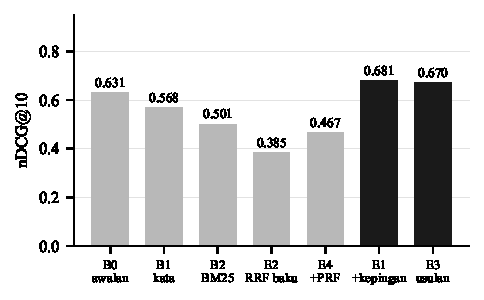
\includegraphics[width=\columnwidth]{gambar1-sistem}
\caption{nDCG@10 tujuh sistem pada 260 kueri uji, korpus 8 entitas. Batang gelap
adalah dua sistem yang memakai kepingan karakter. Jarak E1/E3 terhadap B0 jauh
lebih sempit daripada pada korpus enam entitas.}
\label{fig:sistem}
\end{figure}

Sistem usulan E3 mencapai nDCG@10 0,670 terhadap 0,631 milik baseline pencocokan
awalan. Selisih $+0{,}039$ itu \textbf{tidak mencapai signifikansi}
($p = 0{,}079$; lihat Tabel~\ref{tab:ablasi}).

Perbedaan yang tegas justru muncul pada metrik lain. Baseline B0 meninggalkan
\textbf{15,4\% kueri tanpa hasil sama sekali} --- lebih dari satu dari tujuh
kueri berakhir pada layar kosong --- sedangkan seluruh varian yang memakai
kepingan karakter menurunkannya ke \textbf{0,0\%}. R@10 naik dari 0,594 menjadi
0,743, dan MRR dari 0,725 menjadi 0,780.

\subsection{Ablasi komponen dan signifikansi}

Tabel~\ref{tab:ablasi} memisahkan kontribusi tiap komponen.

\begin{table}[!t]
\caption{Ablasi komponen pada himpunan uji (260 kueri). Selisih nDCG@10, selang
kepercayaan 95\%, dan nilai $p$ dari \emph{paired bootstrap} (5.000 resampel,
\texttt{seed}~$=7$), tanpa koreksi perbandingan berganda.}
\label{tab:ablasi}
\centering
\footnotesize
\begin{tabular}{@{}lrrl@{}}
\toprule
\textbf{Perbandingan} & \textbf{$\Delta$nDCG} & \textbf{CI 95\%} & \textbf{$p$} \\
\midrule
B1 vs B0 \emph{(TF--IDF kata saja)}     & $-0{,}064$ & $[-0{,}117; -0{,}011]$ & 0,021 \\
B2 vs B0 \emph{(BM25 kata saja)}        & $-0{,}130$ & $[-0{,}188; -0{,}075]$ & $<0{,}001$ \\
\textbf{E1 vs B1} \emph{(+ kepingan)}   & $\mathbf{+0{,}114}$ & $[+0{,}073; +0{,}153]$ & $\mathbf{<0{,}001}$ \\
E1 vs B0 \emph{(+ kepingan)}            & $+0{,}050$ & $[+0{,}000; +0{,}097]$ & 0,045 \\
E3 vs E1 \emph{(+ Weighted RRF)}        & $-0{,}011$ & $[-0{,}037; +0{,}014]$ & 0,406 \\
E3 vs E2 \emph{(bobot vs RRF baku)}     & $+0{,}285$ & $[+0{,}259; +0{,}310]$ & $<0{,}001$ \\
E2 vs B0 \emph{(RRF baku saja)}         & $-0{,}246$ & $[-0{,}288; -0{,}205]$ & $<0{,}001$ \\
E4 vs B0 \emph{(perluasan kueri)}       & $-0{,}164$ & $[-0{,}218; -0{,}112]$ & $<0{,}001$ \\
E3 vs B0 \emph{(sistem penuh)}          & $+0{,}039$ & $[-0{,}004; +0{,}082]$ & 0,079 \\
\bottomrule
\end{tabular}
\end{table}

Hasil ablasi tegas dan tidak seimbang, tetapi arahnya berbeda dari yang lazim
diklaim. Mengganti pencocokan awalan dengan TF--IDF token kata saja justru
\emph{memburukkan} hasil ($-0{,}064$; $p = 0{,}021$), dan BM25 lebih buruk lagi
($-0{,}130$; $p < 0{,}001$). Penambahan kepingan karakter di atas TF--IDF kata
menyumbang $+0{,}114$ ($p < 0{,}001$) --- inilah satu-satunya komponen dengan
perolehan besar dan meyakinkan. Namun karena titik awalnya sendiri berada di
bawah B0, sistem hibrida hanya berhasil menyusul dan sedikit melampaui baseline
pencocokan awalan: E1 vs B0 $+0{,}050$ ($p = 0{,}045$, signifikan nominal), dan
E3 vs B0 $+0{,}039$ ($p = 0{,}079$, tidak signifikan).

Penambahan fusi peringkat berbobot tidak menyumbang nDCG sama sekali
($-0{,}011$; $p = 0{,}406$), meskipun ia menaikkan P@1 dari 0,623 ke 0,681 dan
MRR dari 0,737 ke 0,780. Pada himpunan dev, pola itu terukur lebih rinci: MRR
naik bermakna ($+0{,}059$; $p = 0{,}0016$) sementara MAP turun bermakna
($-0{,}059$; $p = 0{,}0082$). Fusi berbobot dengan demikian mengangkat hasil
relevan pertama tetapi memperburuk sisa daftar, dan kedua efek itu saling
meniadakan pada nDCG@10.

Dua komponen jelas merugikan. RRF baku tanpa bobot entitas (E2) menurunkan
nDCG@10 sebesar $0{,}246$ di bawah baseline dan meruntuhkan P@1 ke 0,108; ia
meratakan kontribusi delapan entitas berukuran sangat berbeda sehingga penyedia
layanan yang hanya berisi enam dokumen memperoleh pengaruh setara dengan konsep
yang berisi 4.249 dokumen. Perluasan kueri otomatis (E4) menurunkan nDCG@10
sebesar $0{,}164$ sekaligus melipatgandakan latensi tujuh kali. Komponen ini
dibuang dari sistem akhir.

\subsection{Kinerja per jenis degradasi}

Gambar~\ref{fig:tipe} dan Tabel~\ref{tab:tipe} memecah hasil menurut jenis
gangguan kueri.

\begin{figure}[!t]
\centering
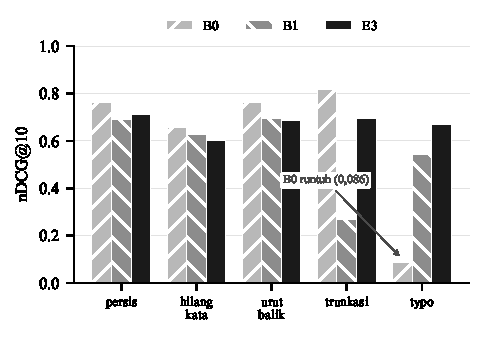
\includegraphics[width=\columnwidth]{gambar2-tipe}
\caption{nDCG@10 menurut jenis degradasi kueri pada himpunan uji. B0 unggul di
empat jenis pertama dan runtuh sepenuhnya pada kesalahan ketik di tengah kata,
karena pencocokan awalan gagal segera setelah huruf pertama yang salah.}
\label{fig:tipe}
\end{figure}

\begin{table}[!t]
\caption{nDCG@10 menurut jenis degradasi kueri (himpunan uji, 260 kueri)}
\label{tab:tipe}
\centering
\footnotesize
\begin{tabular}{@{}lccccc@{}}
\toprule
\textbf{Sistem} & \textbf{persis} & \textbf{hilang} & \textbf{urut} &
\textbf{trunkasi} & \textbf{typo} \\
 & & \textbf{kata} & \textbf{balik} & & \\
\midrule
B0 & \textbf{0,762} & \textbf{0,657} & \textbf{0,760} & \textbf{0,818} & 0,086 \\
B1 & 0,690 & 0,626 & 0,693 & 0,266 & 0,544 \\
E1 & 0,690 & 0,636 & 0,707 & 0,671 & \textbf{0,713} \\
E3 & 0,711 & 0,600 & 0,687 & 0,695 & 0,668 \\
\bottomrule
\end{tabular}
\end{table}

Baseline pencocokan awalan B0 mencapai nDCG@10 0,086 pada kueri dengan kesalahan
ketik --- praktis nol. Perilaku ini konsisten dengan rancangannya: penyaringan
awalan membuang seluruh kandidat begitu satu huruf di tengah kata salah, sehingga
tidak ada yang tersisa untuk diberi skor. Pada empat jenis degradasi lainnya B0
justru \emph{unggul} atas seluruh sistem, termasuk sistem usulan.

Inilah struktur hasil yang menjelaskan angka agregat: keunggulan sistem usulan
terkonsentrasi pada satu jenis kesalahan (typo, 0,668--0,713 vs 0,086), sedangkan
pada empat jenis lain ia membayar harga. Rata-rata keduanya menghasilkan selisih
kecil yang tidak signifikan.

\subsection{Kinerja per entitas --- temuan utama}

Tabel~\ref{tab:entitas} memuat temuan yang paling menjelaskan seluruh naskah ini.

\begin{table*}[!t]
\caption{nDCG@10 menurut entitas sasaran kueri (himpunan uji, 260 kueri).
Kolom diurutkan menurut selisih E3 terhadap B0: manfaat sistem usulan
berbalik tanda antara entitas berciri kamus (kiri) dan entitas instans
per-pasien (kanan).}
\label{tab:entitas}
\centering
\footnotesize
\setlength{\tabcolsep}{11pt}
\begin{tabular}{@{}lcccccccc@{}}
\toprule
\textbf{Sistem} & \textbf{form} & \textbf{obat} & \textbf{konsep} &
\textbf{lokasi} & \textbf{provider} & \textbf{kondisi} &
\textbf{hasil lab} & \textbf{pasien} \\
\midrule
B0 & 0,667 & 0,568 & 0,600 & 0,727 & \textbf{1,000} & \textbf{0,685} & \textbf{0,579} & \textbf{0,710} \\
B1 & 0,772 & 0,614 & 0,602 & 0,603 & \textbf{1,000} & 0,581 & 0,587 & 0,391 \\
E1 & \textbf{1,000} & \textbf{0,800} & 0,723 & 0,718 & \textbf{1,000} & \textbf{0,741} & 0,650 & 0,399 \\
E3 & \textbf{1,000} & \textbf{0,800} & \textbf{0,771} & \textbf{0,785} & \textbf{1,000} & 0,632 & 0,399 & 0,468 \\
\midrule
\emph{E3 $-$ B0} & $+0{,}333$ & $+0{,}232$ & $+0{,}171$ & $+0{,}058$ & $0{,}000$ & $-0{,}053$ & $-0{,}180$ & $-0{,}242$ \\
\bottomrule
\end{tabular}
\end{table*}

Manfaat sistem usulan \textbf{tidak merata dan berbalik tanda}. Pada lima entitas
berciri kamus --- formulir, obat, konsep, lokasi, penyedia layanan --- E3 unggul
atau setara, dengan selisih terbesar $+0{,}333$ pada formulir dan $+0{,}232$ pada
obat. Pada tiga entitas yang berisi instans per-pasien --- kondisi, hasil
laboratorium, dan pasien --- E3 \emph{kalah} dari pencocokan awalan, dengan
defisit terbesar $-0{,}242$ pada pasien dan $-0{,}180$ pada hasil laboratorium.

Pada hasil laboratorium, fusi berbobot memperburuk keadaan secara khusus: E1
mencapai 0,650 sedangkan E3 hanya 0,399. Mekanismenya dapat ditelusuri. Dengan
2.018 dokumen yang hanya memuat 203 judul unik, puluhan dokumen memperoleh skor
kosinus yang identik. Fusi berbasis skor mentah (E1) mempertahankan seluruhnya
pada tingkat skor yang sama, sedangkan RRF memberi mereka peringkat berurutan
$r = 1, 2, \dots, 37$ di dalam entitasnya, sehingga suku $1/(k+r)$ menurun tajam
dan sebagian besar dokumen yang sama sahihnya terdorong keluar dari sepuluh
besar.

\subsection{Sapuan parameter}

Seluruh parameter dikunci pada 100 kueri dev sebelum himpunan uji dijalankan.
Gambar~\ref{fig:sapuan} menyajikan dua sapuan yang paling menentukan.

\begin{figure}[!t]
\centering
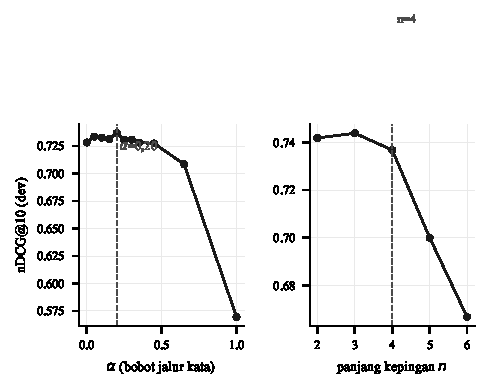
\includegraphics[width=\columnwidth]{gambar3-sapuan}
\caption{Sapuan parameter pada 100 kueri pengembangan, korpus 8 entitas. Kiri:
bobot jalur kata $\alpha$; nilai $\alpha = 0$ (kepingan saja) mencapai 0,728,
sedangkan $\alpha = 1$ (kata saja) anjlok ke 0,570. Kanan: panjang kepingan $n$.}
\label{fig:sapuan}
\end{figure}

Sapuan $\alpha$ mencapai maksimum tepat pada $\alpha = 0{,}20$ (nDCG dev 0,7368),
nilai yang sama dengan yang dikunci pada korpus enam entitas --- sebuah
konfirmasi yang tidak direncanakan. Kedua ujungnya informatif: $\alpha = 1$
(hanya jalur kata) memberi 0,570, sedangkan $\alpha = 0$ (hanya jalur kepingan)
memberi 0,728. Jalur kepingan sendirian mengungguli jalur kata sendirian dengan
selisih besar.

Sapuan panjang kepingan kembali menunjukkan $n = 3$ sedikit unggul (0,7438)
atas $n = 4$ (0,7368), selisih $+0{,}0071$, tetapi kali ini uji bootstrap
menghasilkan $p = 0{,}2806$ dengan CI 95\% $[-0{,}0059; +0{,}0209]$ yang memuat
nol. Berbeda dari korpus enam entitas yang memberi $p = 0{,}0686$
(\emph{borderline}), pada korpus penuh keunggulan $n = 3$ jelas tidak dapat
dibedakan dari derau. Nilai $n = 4$ dipertahankan.

Sapuan $k$ pada RRF (5, 10, 20, 60) menghasilkan rentang 0,7340--0,7396 dan
sapuan $\varepsilon$ (0; 0,05; 0,15; 0,30) menghasilkan 0,7366--0,7387 ---
keduanya di dalam derau. Nilai 20 dan 0,05 dipertahankan. Tidak ada di antara
keempat parameter yang bersumber dari himpunan uji.

\subsection{Perbandingan terhadap pencarian OpenMRS yang sesungguhnya}

Tabel~\ref{tab:b0prime} dan Gambar~\ref{fig:b0prime} membandingkan sistem usulan
terhadap endpoint OpenMRS yang sesungguhnya pada 34 kueri konsep pengembangan.

\begin{table}[!t]
\caption{Perbandingan terhadap pencarian konsep OpenMRS asli (34 kueri konsep
pengembangan). B0$'$ adalah endpoint \emph{fuzzy} Lucene OpenMRS yang dipanggil
langsung.}
\label{tab:b0prime}
\centering
\footnotesize
\begin{tabular}{@{}lccc@{}}
\toprule
\textbf{Sistem} & \textbf{P@1} & \textbf{nDCG@10} & \textbf{\% nol-hasil} \\
\midrule
B0 \emph{(tiruan awalan)}      & 0,588 & 0,499 & 29,4 \\
B1 \emph{(TF--IDF kata)}       & 0,559 & 0,527 & 20,6 \\
B0$'$ \emph{(OpenMRS asli)}    & \textbf{0,912} & 0,733 & \phantom{0}8,8 \\
E1 \emph{(+ kepingan)}         & 0,824 & 0,739 & \phantom{0}\textbf{2,9} \\
\textbf{E3} \emph{(usulan)}    & 0,794 & \textbf{0,788} & \phantom{0}\textbf{2,9} \\
\midrule
\multicolumn{4}{@{}l@{}}{\emph{Uji bootstrap (seed~$=7$, $n=34$):}} \\
\multicolumn{4}{@{}l@{}}{\quad E3 vs B0$'$: $+0{,}055$, CI $[-0{,}043; +0{,}153]$, $p = 0{,}269$} \\
\multicolumn{4}{@{}l@{}}{\quad E3 vs B0\phantom{$'$}: $+0{,}290$, CI $[+0{,}164; +0{,}417]$, $p < 0{,}001$} \\
\multicolumn{4}{@{}l@{}}{\quad B0$'$ vs B0: $+0{,}235$, CI $[+0{,}119; +0{,}359]$, $p = 0{,}0006$} \\
\bottomrule
\end{tabular}
\end{table}

\begin{figure}[!t]
\centering
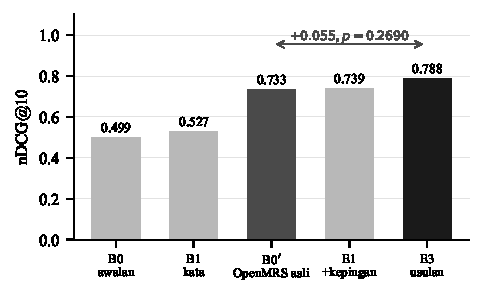
\includegraphics[width=\columnwidth]{gambar4-b0prime}
\caption{nDCG@10 pada 34 kueri konsep pengembangan. Pencarian OpenMRS yang
sesungguhnya (B0$'$) mengungguli tiruan pencocokan awalan kami sendiri (B0)
sebesar $+0{,}235$. Sistem usulan sedikit lebih unggul dari B0$'$, tetapi
selisihnya tidak signifikan.}
\label{fig:b0prime}
\end{figure}

Endpoint OpenMRS asli mengungguli tiruan pencocokan awalan kami sendiri sebesar
$+0{,}235$ nDCG ($p = 0{,}0006$). Dengan kata lain, baseline yang kami bangun
\emph{meremehkan} sistem yang hendak kami bandingkan. Sistem usulan masih di atas
OpenMRS asli, tetapi hanya $+0{,}055$ dengan $p = 0{,}269$ --- \textbf{tidak
signifikan}. Yang bertahan adalah keunggulan pada cakupan: B0$'$ meninggalkan
8,8\% kueri tanpa hasil, sistem usulan 2,9\%.

Dua pemeriksaan validitas dilakukan pada pengukuran ini dan keduanya bersih:
tidak satu pun dari 109 hasil yang dikembalikan endpoint berada di luar korpus
konsep yang kami indeks, dan tidak satu pun dari 34 kueri menghasilkan urutan
berbeda pada dua pemanggilan.

\subsection{Jalur saran ketik}

Tabel~\ref{tab:k2} dan Gambar~\ref{fig:k2} menyajikan hasil evaluasi jalur saran
ketik pada 214 kueri, terpisah dari seluruh angka di atas.

\begin{table}[!t]
\caption{Akurasi saran ketik (214 kueri, korpus 8 entitas). Tidak ada nDCG untuk
jalur ini karena ia tidak menyentuh peringkat.}
\label{tab:k2}
\centering
\footnotesize
\begin{tabular}{@{}lccccc@{}}
\toprule
\textbf{Jenis} & \textbf{$n$} & \textbf{hit@1} & \textbf{hit@3} &
\textbf{hit@6} & \textbf{MRR@6} \\
\midrule
persis            & \phantom{0}52 & 0,962 & 1,000 & 1,000 & 0,981 \\
typo              & \phantom{0}66 & 0,864 & 0,985 & 0,985 & 0,924 \\
trunkasi          & \phantom{0}46 & 0,609 & 0,870 & 0,913 & 0,734 \\
trunkasi\_pendek  & \phantom{0}26 & 0,308 & 0,462 & 0,692 & 0,426 \\
typo\_pendek      & \phantom{0}24 & 0,125 & 0,208 & 0,375 & 0,192 \\
\midrule
\textbf{keseluruhan} & \textbf{214} & \textbf{0,682} & \textbf{0,813} &
\textbf{0,869} & \textbf{0,754} \\
\bottomrule
\end{tabular}
\end{table}

\begin{figure}[!t]
\centering
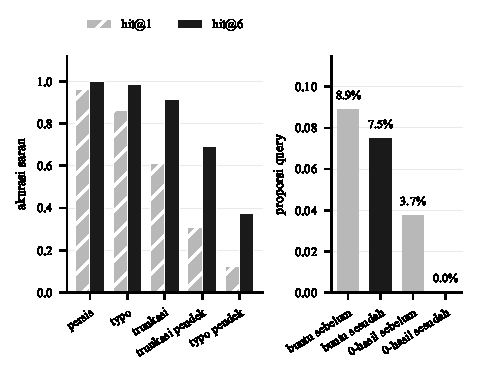
\includegraphics[width=\columnwidth]{gambar5-k2}
\caption{Kiri: akurasi saran menurut jenis degradasi. Kanan: proporsi kueri buntu
dan kueri tanpa hasil, sebelum dan sesudah satu klik pada saran teratas.}
\label{fig:k2}
\end{figure}

Kontrol \emph{persis} mencapai hit@3 sempurna, yang menunjukkan metrik dan
implementasi bekerja sebagaimana mestinya. Jalur saran kuat pada kesalahan ketik
kata utuh (hit@6 0,985) dan memadai pada kata terpotong (0,913), tetapi melemah
tajam pada kueri sangat pendek (\emph{typo\_pendek} hit@1 0,125). Penyebabnya
struktural: Jaccard menghukum kecocokan parsial melalui penyebut gabungan,
sehingga prefiks empat sampai enam huruf dari frasa panjang memiliki himpunan
gabungan yang besar dan kalah dari kata pendek acak yang kebetulan berbagi dua
atau tiga bigram.

Pada metrik interaksi, dari 8,9\% kueri yang buntu, satu klik pada saran teratas
menyelamatkan 15,8\%, menurunkan kebuntuan efektif menjadi 7,5\%. Efek yang
paling jelas ada pada metrik lain: kueri yang mengembalikan nol dokumen turun
dari 3,7\% menjadi 0,0\%. Kami tidak mengklaim jalur ini meningkatkan mutu
peringkat, dan tidak melaporkan nDCG untuknya.

\subsection{Verifikasi silang implementasi dan kinerja modul}

Tabel~\ref{tab:verifikasi} merangkum verifikasi silang antara modul Java yang
berjalan di server OpenMRS dan pipeline Python, keduanya pada korpus 8 entitas
yang sama.

\begin{table}[!t]
\caption{Verifikasi silang Java (live) terhadap Python, 100 kueri dev, korpus 8
entitas. Standar emas identik, diverifikasi melalui SHA-256
\texttt{7ed59a42\dots cd91ee}.}
\label{tab:verifikasi}
\centering
\footnotesize
\setlength{\tabcolsep}{5pt}
\begin{tabular}{@{}lrrr@{}}
\toprule
\textbf{Besaran} & \textbf{Java (live)} & \textbf{Python} & \textbf{Selisih} \\
\midrule
Dokumen           & 8.045 & 8.045 & 0 \\
Surface form      & 35.914 & 35.914 & 0 \\
Indeks            & 17 & 17 & 0 \\
\midrule
nDCG@10 mode b0   & 0,5613 & 0,5613 & 0,0000 \\
nDCG@10 mode b1   & 0,5546 & 0,5534 & 0,0012 \\
nDCG@10 mode e1   & 0,7383 & 0,7371 & 0,0012 \\
nDCG@10 mode e3   & 0,7368 & 0,7368 & 0,0000 \\
\bottomrule
\end{tabular}
\end{table}

Korpus cocok persis. Mode \texttt{b0} dan \texttt{e3} mereproduksi angka Python
tanpa selisih sama sekali. Mode \texttt{b1} dan \texttt{e1} berselisih 0,0012 ---
setara satu kueri yang peringkatnya berbeda. Kedua mode itu memeringkat menurut
skor kosinus mentah, dan pada korpus yang memuat puluhan dokumen berjudul identik
banyak skor bernilai persis sama, sehingga perbedaan pembulatan floating-point
yang sangat kecil dapat membalik urutan pasangan yang seri. Mode \texttt{e3},
yang memeringkat menurut peringkat bilangan bulat alih-alih skor pecahan, kebal
terhadap efek itu dan cocok persis. Kami melaporkan selisih ini apa adanya;
besarannya jauh di bawah selisih antar-sistem mana pun yang dibahas naskah ini.

Latensi diukur melalui header respons pada permintaan berturut-turut. Setelah
100 permintaan pemanasan, 20 permintaan berikutnya memberi p50 42~ms, p95 50~ms,
minimum 39~ms, dan maksimum 63~ms. Angka ini lebih tinggi daripada pada korpus
enam entitas (p95 26~ms), sebanding dengan bertambahnya indeks dari 13 menjadi
17 dan surface form dari 29.320 menjadi 35.914.

Determinisme diverifikasi dengan menjalankan pipeline pada proses terpisah;
seluruh berkas hasil identik pada tingkat bita, kecuali medan waktu pembangunan
indeks. Rangkaian uji unit modul lulus seluruhnya (47 dari 47).

% =============================================================================
\section{Discussion}
\label{sec:diskusi}
% =============================================================================

\subsection{Jawaban atas rumusan masalah}

\textbf{RQ1.} Pada korpus penuh delapan entitas, mesin pencarian terpadu yang
diusulkan mencapai nDCG@10 0,670 terhadap 0,631 milik baseline pencocokan awalan.
Selisih $+0{,}039$ itu \textbf{tidak mencapai signifikansi} ($p = 0{,}079$).
Keunggulan yang nyata dan besar berada pada dimensi lain: proporsi kueri tanpa
hasil turun dari 15,4\% menjadi 0,0\%, R@10 naik 0,149, dan MRR naik 0,055.

\textbf{RQ2.} Hanya satu komponen yang menyumbang perolehan besar dan meyakinkan:
kepingan karakter, $+0{,}114$ nDCG di atas TF--IDF token kata ($p < 0{,}001$).
Fusi peringkat berbobot tidak menyumbang nDCG ($-0{,}011$; $p = 0{,}406$) meski
menaikkan P@1 dan MRR. Dua komponen lain merugikan: RRF tanpa bobot
($-0{,}246$) dan perluasan kueri otomatis ($-0{,}164$).

\textbf{RQ3.} Tidak. Terhadap endpoint pencarian konsep OpenMRS yang
sesungguhnya, selisihnya $+0{,}055$ dengan $p = 0{,}269$ --- tidak signifikan.
Yang bertahan adalah keunggulan cakupan: 2,9\% kueri tanpa hasil dibanding 8,8\%.

\textbf{RQ4.} Ya. Modul membangun tujuh belas indeks dalam 2,08~detik pada saat
mulai dan melayani kueri pada p95 50~ms setelah JVM hangat, tanpa GPU, tanpa
server indeks terpisah, dan tanpa sambungan keluar. Korpusnya cocok persis dengan
pipeline penelitian, dan dua dari empat mode mereproduksi angkanya tanpa selisih.

\subsection{Temuan utama: manfaatnya bergantung pada sifat entitas}

Kontribusi terpenting naskah ini bukan angka agregat, melainkan
Tabel~\ref{tab:entitas}. Manfaat kepingan karakter \textbf{berbalik tanda}
menurut sifat entitas yang diindeks.

Pada entitas berciri kamus --- formulir, obat, konsep, lokasi --- setiap dokumen
memiliki judul yang unik dan bermakna, sering disertai sinonim dan kode. Di sini
kepingan karakter bekerja persis seperti yang diharapkan: ia memulihkan
kecocokan yang hancur oleh satu huruf salah, dan sistem usulan unggul
$+0{,}171$ sampai $+0{,}333$.

Pada entitas berisi instans per-pasien --- hasil laboratorium, kondisi, pasien
--- asumsi itu runtuh. Judul berulang lintas ratusan baris: 2.018 hasil
laboratorium hanya memuat 203 judul unik. Akibatnya, sebuah kueri tidak lagi
memiliki satu jawaban benar melainkan puluhan yang sama sahihnya, dan tugasnya
berubah dari \emph{menemukan entri yang tepat} menjadi \emph{memilih instans yang
tepat} --- tugas yang tidak dapat diselesaikan oleh kecocokan teks, karena
seluruh kandidat memiliki teks yang identik. Pada tugas semacam itu pencocokan
awalan yang mengembalikan sedikit hasil eksak justru lebih menguntungkan menurut
nDCG@10 daripada sistem yang mengembalikan banyak kandidat serupa.

Fusi peringkat berbobot memperburuk keadaan pada kasus ini secara khusus dan
dapat dijelaskan mekanismenya: RRF mengubah skor identik menjadi peringkat
berurutan, dan suku $1/(k+r)$ kemudian mendorong sebagian besar kandidat yang
sama sahihnya keluar dari sepuluh besar. Itu sebabnya E3 (0,399) jauh di bawah
E1 (0,650) pada hasil laboratorium.

Implikasi praktisnya langsung: pada instalasi OpenMRS, jalur kepingan karakter
sebaiknya diterapkan pada entitas kamus, sementara entitas instans per-pasien
lebih baik dilayani pencarian berbasis awalan yang digabungkan dengan penyaring
terstruktur (tanggal, pasien, rentang nilai). Merapikan keduanya di bawah satu
fungsi peringkat, seperti yang dilakukan sistem ini, membayar harga yang terukur.

\subsection{Mengapa angka ini jauh lebih kecil daripada versi enam entitas}

Versi awal penelitian ini mengevaluasi enam entitas dan melaporkan E3 unggul
$+0{,}187$ nDCG atas B0 dengan $p < 0{,}001$. Pada korpus penuh delapan entitas
angka yang sama menjadi $+0{,}039$ dengan $p = 0{,}079$. Penyusutan itu bukan
akibat perubahan algoritma --- parameternya identik, kodenya sama --- melainkan
akibat masuknya dua entitas yang sifatnya berbeda secara mendasar.

Kami menilai versi delapan entitas sebagai versi yang benar, dengan alasan
sederhana: itulah cakupan yang benar-benar diindeks oleh modul yang dipasang
pengguna. Melaporkan angka enam entitas berarti melaporkan sistem yang tidak
dijalankan siapa pun. Bahwa angka yang benar jauh lebih kecil adalah hasil, bukan
alasan untuk kembali ke cakupan yang lebih menguntungkan.

\subsection{Apa yang tetap bertahan}

Tiga klaim bertahan dengan kuat dan tidak bergantung pada cakupan korpus.

\emph{Pertama, penghapusan jalan buntu.} Baseline pencocokan awalan meninggalkan
15,4\% kueri tanpa hasil sama sekali; seluruh varian berkepingan karakter
menurunkannya ke nol. Dalam konteks klinis, layar kosong adalah mode kegagalan
yang berbeda secara kualitatif dari hasil yang buruk --- ia menghentikan alur
kerja, bukan memperlambatnya \cite{hersh2020, natarajan2010}. Ukuran ini tidak
tertangkap oleh nDCG@10, dan justru di sinilah letak nilai praktis metode ini.

\emph{Kedua, ketahanan terhadap kesalahan ketik.} Pada kueri bertipe typo,
pencocokan awalan mencapai 0,086 sementara sistem hibrida mencapai 0,668--0,713.
Perbedaan hampir delapan kali lipat itu adalah manifestasi konkret dari sifat
kepingan karakter yang sudah dikenal pada kepustakaan pencocokan string
aproksimatif \cite{ukkonen1992, kondrak2005} dan perolehan lintas-bahasa
\cite{mcnamee2004}.

\emph{Ketiga, pentingnya pembobotan pada fusi antar-entitas.} RRF tanpa bobot
menurunkan nDCG@10 sebesar 0,246 dan meruntuhkan P@1 ke 0,108. Pembobotan
berbasis indeks global mengembalikan P@1 ke 0,681. Temuan ini menguat, bukan
melemah, pada korpus yang lebih heterogen --- sejalan dengan analisis fungsi fusi
yang menemukan bahwa fusi berbasis peringkat memerlukan pembobotan ketika daftar
sumber memiliki karakteristik yang sangat berbeda \cite{bruch2023, cormack2009}.

\subsection{Pelajaran metodologis: baseline dan korpus yang setia}

Dua kekeliruan metodologis ditemukan dalam penelitian ini sendiri, dan keduanya
bergerak ke arah yang sama --- membesarkan klaim.

\emph{Baseline yang tidak setia.} Kami membangun B0 sebagai tiruan ``pencarian
bawaan OpenMRS''. Ketika endpoint yang sesungguhnya akhirnya dipanggil langsung,
ia mengalahkan tiruan kami sendiri sebesar $+0{,}235$ nDCG. Satu asumsi yang
tidak diuji --- bahwa pencarian OpenMRS bekerja dengan pencocokan awalan,
padahal pencarian konsepnya memakai \emph{fuzzy} berbasis Lucene --- melipatkan
besaran klaim beberapa kali.

\emph{Korpus evaluasi yang tidak setia.} Pipeline penelitian mengindeks enam
entitas sementara modul yang dipasang mengindeks delapan. Selama endpoint REST
instalasi uji mengalami gangguan, ketidakcocokan itu tidak terlihat sama sekali;
ia baru terungkap ketika endpoint pulih dan angka evaluasi live dapat
dibandingkan dengan angka pipeline.

Pelajarannya berlaku umum untuk penelitian yang mengusulkan perbaikan atas sistem
yang sudah berjalan: ukurlah terhadap sistem itu sendiri, pada cakupan data yang
sama dengan yang benar-benar dijalankan. Rekonstruksi dari dokumentasi dan
subhimpunan data yang nyaman keduanya cenderung menguntungkan sistem yang
diusulkan.

Kami juga mencatat bahwa penelitian ini pernah mencemari himpunan ujinya sendiri
melalui sapuan parameter yang keliru dijalankan pada bagian uji. Seluruh angka
sapuan dijalankan ulang pada himpunan pengembangan dan skrip lama diarsipkan.

\subsection{Perbandingan dengan kepustakaan}

Sistem pencarian RME yang matang seperti EMERSE \cite{hanauer2015} dan
Doc'EDS \cite{pressat2022} berfokus pada perolehan dokumen naratif dan
memanfaatkan mesin indeks penuh, sementara pendekatan rekomendasi kueri berbasis
semantik \cite{wu2023} menuntut sumber daya terminologi tambahan. Penelitian
mengenai koreksi ejaan pada domain kesehatan umumnya memperlakukan koreksi
sebagai tugas tersendiri dengan leksikon dan model bahasa
\cite{crowell2004, lai2015, kilicoglu2015}. Kontribusi naskah ini terletak pada
sisi yang berbeda: toleransi salah ketik dicapai \emph{di dalam} fungsi
peringkat, tanpa leksikon koreksi, tanpa model bahasa, dan tanpa mesin indeks
eksternal --- pilihan yang ditentukan oleh batasan penerapan.

Dibandingkan pemeringkat neural \cite{lin2022, khattab2020, formal2021}, hasil
kami jelas bukan kompetisi mutu absolut; kami tidak menguji sistem neural dan
tidak mengklaim keunggulan atasnya. Klaim kami kini bahkan lebih sempit daripada
yang semula direncanakan: pada kelas fasilitas yang menjadi sasaran OpenMRS,
kerugian akibat salah ketik dapat dipulihkan tanpa akselerator dan tanpa
konektivitas, dengan biaya latensi puluhan milidetik --- tetapi perolehan itu
terkonsentrasi pada entitas berciri kamus, dan tidak berlaku merata.

\subsection{Keterbatasan}

\emph{Kueri sintetis.} Kueri dibangkitkan dengan menerapkan lima jenis degradasi
pada judul dokumen, bukan diambil dari log klinisi. Model degradasi ini
didasarkan pada taksonomi kesalahan yang mapan \cite{kukich1992, damerau1964},
tetapi distribusi jenis kesalahan pada kueri nyata hampir pasti berbeda. Karena
sistem usulan unggul hanya pada satu jenis degradasi dari lima, hasil agregat
sangat peka terhadap asumsi distribusi ini --- kelemahan yang lebih menonjol pada
korpus delapan entitas daripada sebelumnya.

\emph{Dua model relevansi dalam satu metrik.} Standar emas memakai tautan
struktural untuk enam entitas dan kesamaan judul untuk dua entitas lainnya.
Menggabungkan keduanya dalam satu angka nDCG melemahkan ketertafsirannya. Kami
melaporkan pemecahan per entitas justru karena alasan itu.

\emph{Kueri pasien dan hasil laboratorium tidak realistis.} Pada praktik nyata,
pencarian pasien dan hasil laboratorium hampir selalu disertai penyaring
terstruktur (identitas, tanggal, jenis pemeriksaan). Eksperimen ini
memperlakukannya sebagai pencarian teks bebas murni, yang menyudutkan seluruh
sistem --- termasuk baseline --- pada tugas yang tidak sepenuhnya mewakili
penggunaan sebenarnya.

\emph{Cakupan B0$'$ sempit.} Baseline yang setia hanya dapat diukur pada 34 kueri
konsep pengembangan, karena OpenMRS tidak menyediakan pencarian tahan salah ketik
untuk tujuh entitas lainnya. Dengan $n = 34$, daya ujinya rendah; ketiadaan
signifikansi pada perbandingan E3 vs B0$'$ tidak boleh dibaca sebagai bukti
ketiadaan perbedaan.

\emph{Skala korpus.} Instalasi yang diuji berisi 4.249 konsep, sedangkan kamus
CIEL penuh berisi sekitar 50.000 konsep. Indeks kepingan berukuran tiga sampai
lima kali indeks kata.

\emph{Indeks statis.} Indeks dibangun satu kali saat modul mulai. Pasien, hasil
laboratorium, atau konsep baru tidak masuk indeks sampai modul dijalankan ulang
--- keterbatasan yang dapat diterima untuk kamus terminologi, tetapi serius untuk
data pasien pada penggunaan produksi.

\emph{Validasi klinis belum dilakukan.} Seluruh pengukuran bersifat berbasis
korpus. Tidak ada studi pengguna dan tidak ada bukti bahwa perubahan nDCG
diterjemahkan menjadi manfaat klinis.

\subsection{Pekerjaan lanjutan}

Temuan utama naskah ini langsung menunjuk arah berikutnya. \emph{Pertama},
memisahkan strategi peringkat menurut sifat entitas --- kepingan karakter untuk
entitas kamus, pencocokan awalan berpenyaring terstruktur untuk entitas instans
--- lalu mengukur apakah pemisahan itu mengungguli fungsi peringkat tunggal.
\emph{Kedua}, memperlakukan kelompok dokumen berjudul sama sebagai satu satuan
peringkat dengan daftar instans di dalamnya, alih-alih sebagai puluhan dokumen
yang bersaing. \emph{Ketiga}, studi pengguna dengan klinisi, karena metrik
berbasis korpus jelas tidak menangkap nilai penghapusan layar kosong.
\emph{Keempat}, evaluasi pada kamus CIEL penuh untuk mengukur perilaku memori
dan latensi pada skala produksi.

\subsection{Simpulan}

Penelitian ini membangun dan mengevaluasi mesin pencarian terpadu lintas-entitas
yang tahan salah ketik untuk OpenMRS, seluruhnya dari teknik perolehan informasi
leksikal klasik, pada korpus yang cakupannya sama persis dengan modul yang
dipasang.

Hasilnya berlapis dan harus dinyatakan lengkap. Pada 260 kueri uji yang
dijalankan satu kali, sistem mencapai nDCG@10 0,670 terhadap 0,631 milik baseline
pencocokan awalan --- selisih yang \textbf{tidak signifikan} ($p = 0{,}079$).
Terhadap pencarian konsep OpenMRS yang sesungguhnya, selisihnya juga tidak
signifikan ($p = 0{,}269$). Klaim peningkatan mutu peringkat, dengan demikian,
tidak dapat dipertahankan pada korpus penuh.

Yang dapat dipertahankan adalah tiga hal lain: kueri tanpa hasil hilang
sepenuhnya (15,4\% menjadi 0,0\%), ketahanan terhadap kesalahan ketik meningkat
hampir delapan kali lipat (0,086 menjadi 0,713), dan implementasinya terbukti
ringan --- tujuh belas indeks dalam 2,08 detik, p95 50~ms, tanpa GPU dan tanpa
sambungan keluar.

Temuan yang paling berguna bagi peneliti berikutnya adalah bahwa manfaat kepingan
karakter \emph{bergantung pada sifat entitas}: besar pada data berciri kamus,
negatif pada data instans per-pasien yang judulnya berulang. Ketergantungan itu
tidak terlihat selama korpus evaluasi lebih sempit daripada korpus yang
sesungguhnya dipasang --- dan itulah alasan paling kuat untuk menyamakan
keduanya sejak awal.

% =============================================================================
%  UCAPAN TERIMA KASIH
% =============================================================================
\section*{Ucapan Terima Kasih}

Penulis berterima kasih kepada komunitas OpenMRS atas ketersediaan kode sumber,
sebaran Reference Application, dan demo data yang menjadi dasar seluruh
eksperimen dalam penelitian ini.

% =============================================================================
%  DAFTAR PUSTAKA
% =============================================================================
\begin{thebibliography}{40}

\bibitem{mamlin2006}
B.~W. Mamlin, P.~G. Biondich, B.~A. Wolfe, H.~Fraser, D.~Jazayeri, C.~Allen,
J.~Miranda, and W.~M. Tierney, ``Cooking up an open source EMR for developing
countries: OpenMRS --- a recipe for successful collaboration,''
\emph{AMIA Annu. Symp. Proc.}, vol.~2006, pp. 529--533, 2006. PMID: 17238397.

\bibitem{seebregts2009}
C.~J. Seebregts, B.~W. Mamlin, P.~G. Biondich, H.~S.~F. Fraser, B.~A. Wolfe,
D.~Jazayeri, C.~Allen, J.~Miranda, E.~Baker, N.~Musinguzi, D.~Kayiwa,
S.~Fourie, N.~Lesh, C.~Kanter, C.~J. Yiannoutsos, and C.~Bailey,
``The OpenMRS Implementers Network,'' \emph{Int. J. Med. Inform.}, vol.~78,
no.~11, pp. 711--720, Nov. 2009, doi: 10.1016/j.ijmedinf.2008.09.005.

\bibitem{fraser2005}
H.~S.~F. Fraser, P.~Biondich, D.~Moodley, S.~Choi, B.~W. Mamlin, and P.~Szolovits,
``Implementing electronic medical record systems in developing countries,''
\emph{Inform. Prim. Care}, vol.~13, no.~2, pp. 83--95, 2005,
doi: 10.14236/jhi.v13i2.585.

\bibitem{muinga2018}
N.~Muinga, S.~Magare, J.~Monda, O.~Kamau, S.~Houston, H.~Fraser, N.~Powell,
M.~English, and C.~Paton, ``Implementing an open source electronic health record
system in Kenyan health care facilities: Case study,'' \emph{JMIR Med. Inform.},
vol.~6, no.~2, p.~e22, Apr. 2018, doi: 10.2196/medinform.8403.

\bibitem{lewis2012}
T.~Lewis, C.~Synowiec, G.~Lagomarsino, and J.~Schweitzer, ``E-health in low- and
middle-income countries: findings from the Center for Health Market
Innovations,'' \emph{Bull. World Health Organ.}, vol.~90, no.~5, pp. 332--340,
May 2012, doi: 10.2471/BLT.11.099820.

\bibitem{natarajan2010}
K.~Natarajan, D.~Stein, S.~Jain, and N.~Elhadad, ``An analysis of clinical
queries in an electronic health record search utility,''
\emph{Int. J. Med. Inform.}, vol.~79, no.~7, pp. 515--522, Jul. 2010,
doi: 10.1016/j.ijmedinf.2010.03.004.

\bibitem{hanauer2015}
D.~A. Hanauer, Q.~Mei, J.~Law, R.~Khanna, and K.~Zheng, ``Supporting information
retrieval from electronic health records: A report of University of Michigan's
nine-year experience in developing and using the Electronic Medical Record
Search Engine (EMERSE),'' \emph{J. Biomed. Inform.}, vol.~55, pp. 290--300,
Jun. 2015, doi: 10.1016/j.jbi.2015.05.003.

\bibitem{lai2015}
K.~H. Lai, M.~Topaz, F.~R. Goss, and L.~Zhou, ``Automated misspelling detection
and correction in clinical free-text records,'' \emph{J. Biomed. Inform.},
vol.~55, pp. 188--195, Jun. 2015, doi: 10.1016/j.jbi.2015.04.008.

\bibitem{crowell2004}
J.~Crowell, Q.~Zeng, L.~Ngo, and E.-M. Lacroix, ``A frequency-based technique to
improve the spelling suggestion rank in medical queries,''
\emph{J. Am. Med. Inform. Assoc.}, vol.~11, no.~3, pp. 179--185, May 2004,
doi: 10.1197/jamia.M1474.

\bibitem{kilicoglu2015}
H.~Kilicoglu, M.~Fiszman, K.~Roberts, and D.~Demner-Fushman, ``An ensemble method
for spelling correction in consumer health questions,''
\emph{AMIA Annu. Symp. Proc.}, vol.~2015, pp. 727--736, 2015. PMID: 26958208.

\bibitem{kukich1992}
K.~Kukich, ``Techniques for automatically correcting words in text,''
\emph{ACM Comput. Surv.}, vol.~24, no.~4, pp. 377--439, Dec. 1992,
doi: 10.1145/146370.146380.

\bibitem{damerau1964}
F.~J. Damerau, ``A technique for computer detection and correction of spelling
errors,'' \emph{Commun. ACM}, vol.~7, no.~3, pp. 171--176, Mar. 1964,
doi: 10.1145/363958.363994.

\bibitem{wagner1974}
R.~A. Wagner and M.~J. Fischer, ``The string-to-string correction problem,''
\emph{J. ACM}, vol.~21, no.~1, pp. 168--173, Jan. 1974,
doi: 10.1145/321796.321811.

\bibitem{ukkonen1992}
E.~Ukkonen, ``Approximate string-matching with $q$-grams and maximal matches,''
\emph{Theor. Comput. Sci.}, vol.~92, no.~1, pp. 191--211, Jan. 1992,
doi: 10.1016/0304-3975(92)90143-4.

\bibitem{kondrak2005}
G.~Kondrak, ``N-gram similarity and distance,'' in \emph{String Processing and
Information Retrieval (SPIRE 2005)}, Lecture Notes in Computer Science,
vol.~3772, Berlin, Germany: Springer, 2005, pp. 115--126,
doi: 10.1007/11575832\_13.

\bibitem{mcnamee2004}
P.~McNamee and J.~Mayfield, ``Character $n$-gram tokenization for European
language text retrieval,'' \emph{Inf. Retr.}, vol.~7, no.~1--2, pp. 73--97,
Jan. 2004, doi: 10.1023/B:INRT.0000009441.78971.be.

\bibitem{boytsov2011}
L.~Boytsov, ``Indexing methods for approximate dictionary searching: Comparative
analysis,'' \emph{ACM J. Exp. Algorithmics}, vol.~16, art.~1.1, May 2011,
doi: 10.1145/1963190.1963191.

\bibitem{salton1975}
G.~Salton, A.~Wong, and C.~S. Yang, ``A vector space model for automatic
indexing,'' \emph{Commun. ACM}, vol.~18, no.~11, pp. 613--620, Nov. 1975,
doi: 10.1145/361219.361220.

\bibitem{salton1988}
G.~Salton and C.~Buckley, ``Term-weighting approaches in automatic text
retrieval,'' \emph{Inf. Process. Manage.}, vol.~24, no.~5, pp. 513--523, 1988,
doi: 10.1016/0306-4573(88)90021-0.

\bibitem{sparckjones1972}
K.~Sp\"{a}rck Jones, ``A statistical interpretation of term specificity and its
application in retrieval,'' \emph{J. Documentation}, vol.~28, no.~1, pp. 11--21,
Jan. 1972, doi: 10.1108/eb026526.

\bibitem{robertson2004}
S.~Robertson, ``Understanding inverse document frequency: on theoretical
arguments for IDF,'' \emph{J. Documentation}, vol.~60, no.~5, pp. 503--520,
Oct. 2004, doi: 10.1108/00220410410560582.

\bibitem{robertson2009}
S.~Robertson and H.~Zaragoza, ``The probabilistic relevance framework: BM25 and
beyond,'' \emph{Found. Trends Inf. Retr.}, vol.~3, no.~4, pp. 333--389, 2009,
doi: 10.1561/1500000019.

\bibitem{zobel1998}
J.~Zobel and A.~Moffat, ``Exploring the similarity space,''
\emph{ACM SIGIR Forum}, vol.~32, no.~1, pp. 18--34, Apr. 1998,
doi: 10.1145/281250.281256.

\bibitem{cormack2009}
G.~V. Cormack, C.~L.~A. Clarke, and S.~B\"{u}ttcher, ``Reciprocal rank fusion
outperforms Condorcet and individual rank learning methods,'' in \emph{Proc.
32nd Int. ACM SIGIR Conf. Research and Development in Information Retrieval},
Boston, MA, USA, 2009, pp. 758--759, doi: 10.1145/1571941.1572114.

\bibitem{bruch2023}
S.~Bruch, S.~Gai, and A.~Ingber, ``An analysis of fusion functions for hybrid
retrieval,'' \emph{ACM Trans. Inf. Syst.}, vol.~42, no.~1, art.~20, pp. 1--35,
Jan. 2024, doi: 10.1145/3596512.

\bibitem{ruthven2003}
I.~Ruthven, ``Re-examining the potential effectiveness of interactive query
expansion,'' in \emph{Proc. 26th Annu. Int. ACM SIGIR Conf. Research and
Development in Information Retrieval}, Toronto, ON, Canada, 2003, pp. 213--220,
doi: 10.1145/860435.860475.

\bibitem{jaccard1912}
P.~Jaccard, ``The distribution of the flora in the alpine zone,''
\emph{New Phytologist}, vol.~11, no.~2, pp. 37--50, Feb. 1912,
doi: 10.1111/j.1469-8137.1912.tb05611.x.

\bibitem{jarvelin2002}
K.~J\"{a}rvelin and J.~Kek\"{a}l\"{a}inen, ``Cumulated gain-based evaluation of IR
techniques,'' \emph{ACM Trans. Inf. Syst.}, vol.~20, no.~4, pp. 422--446,
Oct. 2002, doi: 10.1145/582415.582418.

\bibitem{efron1979}
B.~Efron, ``Bootstrap methods: Another look at the jackknife,''
\emph{Ann. Statist.}, vol.~7, no.~1, pp. 1--26, Jan. 1979,
doi: 10.1214/aos/1176344552.

\bibitem{smucker2007}
M.~D. Smucker, J.~Allan, and B.~Carterette, ``A comparison of statistical
significance tests for information retrieval evaluation,'' in \emph{Proc. 16th
ACM Conf. Information and Knowledge Management}, Lisbon, Portugal, 2007,
pp. 623--632, doi: 10.1145/1321440.1321528.

\bibitem{sakai2006}
T.~Sakai, ``Evaluating evaluation metrics based on the bootstrap,'' in
\emph{Proc. 29th Annu. Int. ACM SIGIR Conf. Research and Development in
Information Retrieval}, Seattle, WA, USA, 2006, pp. 525--532,
doi: 10.1145/1148170.1148261.

\bibitem{hersh2020}
W.~Hersh, \emph{Information Retrieval: A Biomedical and Health Perspective},
4th~ed. Cham, Switzerland: Springer, 2020,
doi: 10.1007/978-3-030-47686-1.

\bibitem{mcdonald2003}
C.~J. McDonald, S.~M. Huff, J.~G. Suico, G.~Hill, D.~Leavelle, R.~Aller,
A.~Forrey, K.~Mercer, G.~DeMoor, J.~Hook, W.~Williams, J.~Case, and P.~Maloney,
``LOINC, a universal standard for identifying laboratory observations: A 5-year
update,'' \emph{Clin. Chem.}, vol.~49, no.~4, pp. 624--633, Apr. 2003,
doi: 10.1373/49.4.624.

\bibitem{lin2022}
J.~Lin, R.~Nogueira, and A.~Yates, \emph{Pretrained Transformers for Text
Ranking: BERT and Beyond}, Synthesis Lectures on Human Language Technologies.
Cham, Switzerland: Springer, 2022, doi: 10.1007/978-3-031-02181-7.

\bibitem{khattab2020}
O.~Khattab and M.~Zaharia, ``ColBERT: Efficient and effective passage search via
contextualized late interaction over BERT,'' in \emph{Proc. 43rd Int. ACM SIGIR
Conf. Research and Development in Information Retrieval}, 2020, pp. 39--48,
doi: 10.1145/3397271.3401075.

\bibitem{formal2021}
T.~Formal, B.~Piwowarski, and S.~Clinchant, ``SPLADE: Sparse lexical and
expansion model for first stage ranking,'' in \emph{Proc. 44th Int. ACM SIGIR
Conf. Research and Development in Information Retrieval}, 2021, pp. 2288--2292,
doi: 10.1145/3404835.3463098.

\bibitem{strubell2019}
E.~Strubell, A.~Ganesh, and A.~McCallum, ``Energy and policy considerations for
deep learning in NLP,'' in \emph{Proc. 57th Annu. Meeting Assoc. Computational
Linguistics}, Florence, Italy, 2019, pp. 3645--3650,
doi: 10.18653/v1/P19-1355.

\bibitem{pressat2022}
T.~Pressat-Laffouilh\`{e}re, P.~Balay\'{e}, B.~Dahamna, R.~Lelong, K.~Billey,
S.~J. Darmoni, and J.~Grosjean, ``Evaluation of Doc'EDS: a French semantic search
tool to query health documents from a clinical data warehouse,''
\emph{BMC Med. Inform. Decis. Mak.}, vol.~22, art.~34, Feb. 2022,
doi: 10.1186/s12911-022-01762-4.

\bibitem{wu2023}
D.~T.~Y. Wu, D.~Hanauer, P.~Murdock, V.~G.~V. Vydiswaran, Q.~Mei, and K.~Zheng,
``Developing a semantically based query recommendation for an electronic medical
record search engine: Query log analysis and design implications,''
\emph{JMIR Form. Res.}, vol.~7, p.~e45376, 2023, doi: 10.2196/45376.

\end{thebibliography}

% =============================================================================
%  LAMPIRAN -- halaman lampiran diletakkan paling bawah, sesudah daftar pustaka.
%  Tautan Google Drive diisi pada blok "TAUTAN" di kepala lampiran.tex.
% =============================================================================
%% ---------------------------------------------------------------------------
%%  lampiran.tex -- halaman lampiran, disisipkan di bagian paling bawah naskah.
%%
%%  Dipanggil dari main.tex dengan:   %% ---------------------------------------------------------------------------
%%  lampiran.tex -- halaman lampiran, disisipkan di bagian paling bawah naskah.
%%
%%  Dipanggil dari main.tex dengan:   %% ---------------------------------------------------------------------------
%%  lampiran.tex -- halaman lampiran, disisipkan di bagian paling bawah naskah.
%%
%%  Dipanggil dari main.tex dengan:   \input{lampiran}
%%  tepat sebelum \end{document}, sesudah daftar pustaka.
%%
%%  >>> YANG PERLU ANDA ISI ADA DI BLOK "TAUTAN" DI BAWAH INI. <<<
%%      Ganti isi tiga makro berikut, lalu kompilasi ulang. Tidak ada tempat
%%      lain yang perlu disentuh -- seluruh tabel di bawah membaca makro ini.
%% ---------------------------------------------------------------------------

% ===== TAUTAN — ISI DI SINI =================================================

% Repositori GitHub (sudah terisi; ubah kalau repo dipindahkan).
\newcommand{\tautanRepo}{https://github.com/stephenprasetyachrismawan/openmrs-tfidf-ngram}

% Google Drive — kumpulan PPT progress. Ganti teks di dalam kurung kurawal.
\newcommand{\tautanPPT}{\textit{[tempelkan tautan Google Drive di sini]}}

% Google Drive — demo aplikasi (rekaman layar / berkas demo).
\newcommand{\tautanDemo}{\textit{[tempelkan tautan Google Drive di sini]}}

% ===== AKHIR BLOK TAUTAN ====================================================



% Judul bagian lampiran. Tidak memakai \section* bawaan ieeecolor.cls
% karena spasi vertikalnya dirancang untuk tata letak dua kolom dan
% meninggalkan lubang besar pada halaman satu kolom.
\newcommand{\lampiransec}[2]{%
  \par\addvspace{3ex}%
  \noindent{\large\bfseries Lampiran #1\quad #2}%
  \par\addvspace{1.2ex}%
  \noindent\ignorespaces}

\newpage
\onecolumn
\raggedbottom   % kelas IEEE memakai \flushbottom;
                % pada halaman lampiran yang isinya sedikit, itu meregangkan
                % jarak antar-paragraf sampai memenuhi tinggi halaman.

\begin{center}
{\Large\bfseries LAMPIRAN}\\[2pt]
{\normalsize Pencarian Terpadu Tahan Salah Ketik pada OpenMRS}
\end{center}

\vspace{1.5ex}

\noindent
Lampiran ini memuat seluruh tautan ke berkas pendukung penelitian: kode sumber,
data, tutorial menjalankan, panduan pengguna, dan bahan presentasi. Seluruh
berkas yang dapat dipublikasikan berada pada satu repositori GitHub; berkas
yang berukuran besar atau tidak cocok disimpan di repositori kode (rekaman
demo, kumpulan slide) berada pada Google Drive dan tautannya dicantumkan di
Lampiran~B.

% ---------------------------------------------------------------------------
\lampiransec{A}{Repositori Kode Sumber dan Berkas Pendukung}

\noindent
\textbf{Repositori utama:} \url{\tautanRepo}

\vspace{1ex}
\noindent
Seluruh butir pada tabel berikut berada di dalam repositori tersebut. Kolom
``Lokasi'' adalah lintasan relatif terhadap akar repositori.

\vspace{1ex}
\renewcommand{\arraystretch}{1.25}
\begin{longtable}{@{}p{0.28\textwidth}p{0.27\textwidth}p{0.41\textwidth}@{}}
\toprule
\textbf{Butir lampiran} & \textbf{Lokasi di repositori} & \textbf{Keterangan} \\
\midrule
\endfirsthead
\multicolumn{3}{@{}l}{\footnotesize\itshape Lampiran A, lanjutan}\\
\toprule
\textbf{Butir lampiran} & \textbf{Lokasi di repositori} & \textbf{Keterangan} \\
\midrule
\endhead
\midrule
\multicolumn{3}{r@{}}{\footnotesize\itshape bersambung ke halaman berikutnya}\\
\endfoot
\bottomrule
\endlastfoot

\textbf{Kode sumber modul OpenMRS} &
\texttt{backend/} \newline
\texttt{~~openmrs-module-} \newline
\texttt{~~tfidf-search/} &
Modul Java (\texttt{.omod}). Berisi seluruh algoritma K1--K6: normalisasi,
tokenisasi kata dan kepingan karakter, pembobotan \emph{ltc}, fusi tingkat
satu, \emph{Weighted RRF}, baseline B0, jalur saran ketik, serta dua endpoint
REST. Dilengkapi 47 uji unit. \\

\textbf{Kode sumber antarmuka} &
\texttt{frontend/} \newline
\texttt{~~esm-unified-search/} &
Microfrontend (ESM) untuk OpenMRS Reference Application~3: halaman
``Pencarian Terpadu'', halaman ``Perbandingan Pencarian'', dan panel
evaluasi. \\

\textbf{Kode eksperimen} &
\texttt{riset/} &
Implementasi rujukan Python untuk seluruh angka pada naskah:
\texttt{eksperimen2.py} (sistem B0--E4, himpunan uji),
\texttt{eksperimen3\_baseline\_asli.py} (baseline B0$'$),
\texttt{eksperimen\_k2.py} (jalur saran ketik),
\texttt{sapuan\_dev.py} dan \texttt{sapuan\_alpha\_dev.py} (sapuan parameter). \\

\textbf{Dataset / basis data} &
\texttt{riset/data/*.jsonl} \newline
\texttt{riset/ekspor\_*.sql} &
Korpus hasil ekspor dari basis data OpenMRS dalam format JSON Lines
(\texttt{konsep}, \texttt{obat}, \texttt{pasien}, \texttt{lain},
\texttt{hasillab}, \texttt{kondisi}), beserta kueri SQL yang dipakai untuk
mengekspornya sehingga dapat dibangkitkan ulang dari instalasi OpenMRS mana
pun. \\

\textbf{Berkas hasil eksperimen} &
\texttt{riset/hasil4/} \dots \texttt{riset/hasil6/} &
Keluaran mentah tiap eksperimen (\texttt{hasil.json},
\texttt{per\_query.json}, \texttt{ringkasan.csv}, \texttt{laporan.md}).
Pemetaan berkas ke tabel dan gambar naskah ada pada Lampiran~F. \\

\textbf{Tutorial menjalankan kode} &
\texttt{README.md} &
Panduan lengkap dari nol: prasyarat, penyalaan stack Docker, pembangunan
modul, pemasangan, verifikasi, sampai halaman terbuka di peramban. Disertai
bagian penanganan galat yang sering muncul. \\

\textbf{Panduan reproduksi hasil} &
\texttt{docs/reproduksi.md} &
Sembilan langkah untuk mengulang seluruh angka penelitian, masing-masing
dengan kriteria ``cara tahu berhasil'' yang dapat diperiksa. \\

\textbf{Panduan pengguna} &
\texttt{docs/panduan-pengguna.md} &
Cara memakai halaman Pencarian Terpadu, halaman Perbandingan Pencarian,
kotak saran ketik, dan panel evaluasi dari sudut pandang pengguna akhir. \\

\textbf{Spesifikasi algoritma} &
\texttt{docs/algoritma.md} &
Spesifikasi K1--K6, baseline B0, dan jalur saran ketik K2, cukup rinci untuk
diimplementasikan ulang tanpa menebak. \\

\textbf{Kontrak data} &
\texttt{docs/kontrak-data.md} &
Bentuk dokumen virtual yang menyatukan delapan entitas OpenMRS; wajib diikuti
persis bila menambahkan entitas baru. \\

\textbf{Catatan keputusan} &
\texttt{docs/keputusan.md} &
Seluruh keputusan rancangan dan temuan penelitian secara kronologis, termasuk
kekeliruan yang ditemukan dan cara memperbaikinya. Rujukan utama untuk
pengembangan lanjutan. \\

\textbf{Fakta lingkungan} &
\texttt{docs/lingkungan.md} &
Versi platform terverifikasi, alamat, kredensial basis data, jumlah baris
tabel, dan jebakan lingkungan yang sudah terdokumentasi. \\

\textbf{Aturan proyek} &
\texttt{CLAUDE.md} &
Sepuluh aturan yang mengikat seluruh perubahan kode dan dokumen, termasuk
aturan determinisme dan larangan mengubah angka hasil. \\

\textbf{Proposal penelitian} &
\texttt{docs/proposal.html} &
Proposal lengkap beserta \emph{mockup} interaktif dan contoh perhitungan. \\

\textbf{Naskah artikel ini} &
\texttt{article/} &
Sumber \LaTeX{} naskah, skrip pembangun gambar, dan berkas hasil kompilasi. \\

\end{longtable}

% ---------------------------------------------------------------------------
\vspace{3ex}
\lampiransec{B}{Tautan Berkas Pendukung Eksternal}

\noindent
Berkas berikut berada di Google Drive karena ukurannya tidak sesuai untuk
disimpan pada repositori kode.

\vspace{1ex}
\renewcommand{\arraystretch}{1.6}
\begin{tabular}{@{}p{0.24\textwidth}p{0.72\textwidth}@{}}
\toprule
\textbf{Berkas} & \textbf{Tautan} \\
\midrule

\textbf{Kumpulan PPT Progress} \newline
{\footnotesize Seluruh slide laporan kemajuan penelitian, berurutan menurut
tanggal.} &
\tautanPPT \\

\textbf{Demo Aplikasi} \newline
{\footnotesize Rekaman layar modul yang berjalan: kueri gagal pada kotak
pencarian bawaan, kueri yang sama berhasil pada sistem usulan.} &
\tautanDemo \\

\bottomrule
\end{tabular}

\vspace{1.5ex}
\noindent
{\footnotesize \textbf{Catatan bagi penulis:} kedua tautan di atas diisi pada
blok \texttt{TAUTAN} di kepala berkas \texttt{article/lampiran.tex}
(makro \texttt{\textbackslash tautanPPT} dan \texttt{\textbackslash
tautanDemo}). Tidak perlu mengubah tabel ini.}

% ---------------------------------------------------------------------------
\vspace{3ex}
\lampiransec{C}{Peta Isi Repositori}

\begin{verbatim}
openmrs-tfidf-ngram/
|
+-- README.md                 tutorial lengkap menjalankan dari nol
+-- CLAUDE.md                 aturan proyek yang mengikat
|
+-- backend/openmrs-module-tfidf-search/
|   +-- api/                  algoritma inti + 47 uji unit
|   |   +-- src/main/java/org/openmrs/module/unifiedsearch/
|   |   |   +-- TextNormalizer.java        normalisasi teks
|   |   |   +-- Tokenizer.java             token kata + kepingan karakter
|   |   |   +-- TfIdfIndex.java            indeks terbalik, pembobotan ltc
|   |   |   +-- FusionSearch.java          fusi tingkat 1 (alpha)
|   |   |   +-- WeightedRrf.java           fusi tingkat 2 (Weighted RRF)
|   |   |   +-- OpenMrsHeuristic.java      baseline B0
|   |   |   +-- BigramJaccardSuggester.java  jalur saran ketik
|   |   |   +-- RankingEngine.java         pemilih mode b0/b1/e1/e3
|   |   |   +-- IndexBuilder.java          pembangunan 13 indeks saat startup
|   |   |   +-- EvalService.java           endpoint evaluasi
|   |   |   +-- source/                    proyeksi 8 tabel OpenMRS
|   |   +-- src/main/resources/gold-dev-100.json   standar emas 100 kueri dev
|   +-- omod/                 lapisan web: REST controller, halaman JSP
|
+-- frontend/esm-unified-search/   microfrontend RefApp 3
|
+-- riset/                    eksperimen Python
|   +-- eksperimen2.py                sistem B0-E4, himpunan uji 180 kueri
|   +-- eksperimen3_baseline_asli.py  baseline B0' (OpenMRS asli)
|   +-- eksperimen_k2.py              jalur saran ketik
|   +-- sapuan_dev.py                 sapuan NGRAM / K_RRF / EPS
|   +-- sapuan_alpha_dev.py           sapuan ALPHA
|   +-- data/*.jsonl                  korpus hasil ekspor
|   +-- ekspor_*.sql                  kueri SQL pembangkit korpus
|   +-- hasil4..hasil6/               keluaran mentah tiap eksperimen
|
+-- docs/                     dokumentasi
|   +-- reproduksi.md         9 langkah mengulang hasil
|   +-- panduan-pengguna.md   panduan pengguna akhir
|   +-- algoritma.md          spesifikasi K1-K6 + B0 + K2
|   +-- kontrak-data.md       bentuk dokumen virtual
|   +-- keputusan.md          catatan keputusan dan temuan, kronologis
|   +-- lingkungan.md         versi, alamat, kredensial, jebakan
|   +-- proposal.html         proposal + mockup interaktif
|
+-- scripts/                  otomasi pemasangan (PowerShell)
|   +-- pasang-modul.ps1      build .omod -> salin -> restart -> tunggu sehat
|   +-- pasang-esm.ps1        build ESM -> sisipkan ke importmap
|   +-- verify-openmrs.ps1    pemeriksaan kesehatan menyeluruh
|
+-- article/                  naskah artikel ini
|   +-- main.tex, lampiran.tex, referensi.bib
|   +-- gambar/buat_gambar.py  membangun gambar dari berkas hasil
|
+-- tugas/                    14 berkas tugas berurutan, masing-masing
                              dengan kriteria uji "Selesai kalau"
\end{verbatim}

% ---------------------------------------------------------------------------
\newpage
\lampiransec{D}{Ringkasan Langkah Menjalankan}

\noindent
Ringkasan ini memuat perintah intinya saja. Penjelasan lengkap setiap langkah,
termasuk cara memastikan langkah itu berhasil dan penanganan galat yang sering
muncul, ada pada \texttt{README.md} di akar repositori.

\vspace{1ex}
\noindent\textbf{Prasyarat:} Docker Desktop, Git, JDK~17, Node.js~20+,
Python~3.9+, dan PowerShell (Windows). Rincian versi terverifikasi ada pada
\texttt{docs/lingkungan.md}.

\vspace{1.5ex}
\renewcommand{\arraystretch}{1.2}
\begin{tabular}{@{}p{0.05\textwidth}p{0.40\textwidth}p{0.51\textwidth}@{}}
\toprule
\textbf{No.} & \textbf{Langkah} & \textbf{Perintah} \\
\midrule
1 & Klon repositori penelitian &
\texttt{git clone https://github.com/} \newline
\texttt{~~stephenprasetyachrismawan/} \newline
\texttt{~~openmrs-tfidf-ngram.git} \\
2 & Klon stack Docker OpenMRS sejajar dengan repositori penelitian &
\texttt{git clone https://github.com/} \newline
\texttt{openmrs/openmrs-distro-} \newline
\texttt{referenceapplication.git} \\
3 & Nyalakan stack (tanpa \texttt{-p}) &
\texttt{cd openmrs-distro-referenceapplication} \newline
\texttt{docker compose up -d} \\
4 & Tunggu empat kontainer sehat &
\texttt{docker ps} \\
5 & Bangun dan pasang modul backend &
\texttt{.\textbackslash scripts\textbackslash pasang-modul.ps1} \\
6 & Bangun dan pasang antarmuka ESM &
\texttt{.\textbackslash scripts\textbackslash pasang-esm.ps1} \\
7 & Verifikasi menyeluruh &
\texttt{.\textbackslash scripts\textbackslash verify-openmrs.ps1} \\
8 & Buka di peramban &
\texttt{http://127.0.0.1/openmrs/spa/} \newline
\texttt{unified-search} \\
\bottomrule
\end{tabular}

\vspace{2ex}
\noindent
\textbf{Peringatan lingkungan.} Seluruh alamat memakai \texttt{http://127.0.0.1},
\emph{bukan} \texttt{localhost}. Pada sebagian mesin Windows, \texttt{localhost}
teresolusi ke IPv6 \texttt{::1} yang mungkin dikuasai server lain, sehingga
seluruh lintasan \texttt{/openmrs/\dots} mengembalikan 404. Bila muncul halaman
bawaan Apache, yang salah adalah alamatnya, bukan modulnya.

\vspace{1ex}
\noindent
\textbf{Kredensial demo bawaan:} \texttt{admin} / \texttt{Admin123}.

% ---------------------------------------------------------------------------
\vspace{3ex}
\lampiransec{E}{Antarmuka REST Modul}

\noindent
Basis alamat: \texttt{http://127.0.0.1/openmrs/ws/rest/v1/unifiedsearch}

\vspace{1.5ex}
\renewcommand{\arraystretch}{1.3}
\begin{tabular}{@{}p{0.20\textwidth}p{0.34\textwidth}p{0.42\textwidth}@{}}
\toprule
\textbf{Endpoint} & \textbf{Parameter} & \textbf{Keterangan} \\
\midrule

\texttt{GET /unifiedsearch} &
\texttt{q} (wajib) \newline
\texttt{mode} = \texttt{b0} $|$ \texttt{b1} $|$ \texttt{e1} $|$ \texttt{e3}
  (bawaan \texttt{e3}) \newline
\texttt{limit} (bawaan 10) \newline
\texttt{entitas} (opsional) &
Pencarian terpadu. Parameter \texttt{mode} memilih sistem, sehingga kontribusi
tiap komponen dapat diukur ulang kapan saja tanpa mengubah kode. \\

\texttt{GET /unifiedsearch/} \newline \texttt{saran} &
\texttt{q} (wajib) \newline
\texttt{limit} (bawaan 6) &
Saran ketik ``Maksud Anda'' berbasis Jaccard bigram. Jalur terpisah; tidak
menyentuh peringkat. Hasil berjenis pasien, hasil laboratorium, dan kondisi
disaring menurut privilese \texttt{View Patients} pemanggil. \\

\texttt{GET /unifiedsearch/} \newline \texttt{eval} &
\texttt{mode} (bawaan \texttt{e3}) &
Menjalankan evaluasi atas 100 kueri pengembangan dan mengembalikan P@1, P@5,
R@10, MRR, MAP, nDCG@10, serta proporsi kueri tanpa hasil. Jawaban menyertakan
\texttt{gold\_sha256} agar standar emas yang dipakai dapat dicocokkan. \\

\bottomrule
\end{tabular}

\vspace{1.5ex}
\noindent
Setiap jawaban menyertakan tajuk \texttt{X-Unifiedsearch-Waktu-Ms} berisi waktu
pemrosesan. Waktu sengaja ditempatkan pada tajuk, bukan pada badan JSON, agar
dua panggilan yang sama menghasilkan badan jawaban yang identik pada tingkat
bita --- syarat pengujian determinisme.

\vspace{1.5ex}
\noindent\textbf{Contoh pemanggilan:}
\begin{verbatim}
curl -u admin:Admin123 \
  "http://127.0.0.1/openmrs/ws/rest/v1/unifiedsearch?q=diabete%20melitus&mode=e3"
\end{verbatim}

% ---------------------------------------------------------------------------
\vspace{2ex}
\lampiransec{F}{Pemetaan Berkas Hasil ke Tabel dan Gambar Naskah}

\noindent
Tidak ada angka pada naskah ini yang diketik ulang secara manual ke dalam
gambar. Skrip \texttt{article/gambar/buat\_gambar.py} membaca berkas hasil
di bawah dan membangun ulang seluruh gambar; bila eksperimen dijalankan ulang
dan angkanya berubah, gambarnya ikut berubah.

\vspace{1.5ex}
\renewcommand{\arraystretch}{1.25}
\begin{tabular}{@{}p{0.26\textwidth}p{0.30\textwidth}p{0.40\textwidth}@{}}
\toprule
\textbf{Bagian naskah} & \textbf{Berkas sumber} & \textbf{Cakupan} \\
\midrule
Tabel~\ref{tab:utama}, \ref{tab:ablasi}, \ref{tab:tipe}, \ref{tab:entitas};
Gambar~\ref{fig:sistem}, \ref{fig:tipe} &
\texttt{riset/hasil6/hasil.json} &
260 kueri uji, korpus 8 entitas, sekali jalan, parameter terkunci \\

Gambar~\ref{fig:sapuan} &
\texttt{riset/hasil6/sapuan\_dev.json} &
Sapuan $\alpha$, $n$, $k$, $\varepsilon$ pada 100 kueri pengembangan \\

Tabel~\ref{tab:b0prime}; Gambar~\ref{fig:b0prime} &
\texttt{riset/hasil4/hasil.json} &
34 kueri konsep, baseline B0$'$ (endpoint OpenMRS asli) \\

Tabel~\ref{tab:k2}; Gambar~\ref{fig:k2} &
\texttt{riset/hasil5/hasil.json} &
214 kueri, jalur saran ketik, korpus 8 entitas \\

Tabel~\ref{tab:verifikasi}, angka latensi dan determinisme &
\texttt{docs/keputusan.md} bagian C1--C4, F1--F2 &
Verifikasi silang Java--Python dan pengukuran kinerja modul \\
\bottomrule
\end{tabular}

\vspace{2ex}
\noindent
\textbf{Cara membangkitkan ulang seluruh angka:} jalankan
\texttt{python riset/eksperimen2.py} (himpunan uji),
\texttt{python riset/eksperimen3\_baseline\_asli.py} (baseline B0$'$, perlu
stack Docker berjalan), dan \texttt{python riset/eksperimen\_k2.py}
(jalur saran ketik), lalu \texttt{python article/gambar/buat\_gambar.py} untuk
membangun ulang gambar. Seluruh skrip deterministik: benih acak dipatok,
pengurutan memakai kunci majemuk, dan iterasi himpunan selalu diurutkan lebih
dahulu, sehingga dua proses terpisah menghasilkan berkas yang identik pada
tingkat bita.

\twocolumn

%%  tepat sebelum \end{document}, sesudah daftar pustaka.
%%
%%  >>> YANG PERLU ANDA ISI ADA DI BLOK "TAUTAN" DI BAWAH INI. <<<
%%      Ganti isi tiga makro berikut, lalu kompilasi ulang. Tidak ada tempat
%%      lain yang perlu disentuh -- seluruh tabel di bawah membaca makro ini.
%% ---------------------------------------------------------------------------

% ===== TAUTAN — ISI DI SINI =================================================

% Repositori GitHub (sudah terisi; ubah kalau repo dipindahkan).
\newcommand{\tautanRepo}{https://github.com/stephenprasetyachrismawan/openmrs-tfidf-ngram}

% Google Drive — kumpulan PPT progress. Ganti teks di dalam kurung kurawal.
\newcommand{\tautanPPT}{\textit{[tempelkan tautan Google Drive di sini]}}

% Google Drive — demo aplikasi (rekaman layar / berkas demo).
\newcommand{\tautanDemo}{\textit{[tempelkan tautan Google Drive di sini]}}

% ===== AKHIR BLOK TAUTAN ====================================================



% Judul bagian lampiran. Tidak memakai \section* bawaan ieeecolor.cls
% karena spasi vertikalnya dirancang untuk tata letak dua kolom dan
% meninggalkan lubang besar pada halaman satu kolom.
\newcommand{\lampiransec}[2]{%
  \par\addvspace{3ex}%
  \noindent{\large\bfseries Lampiran #1\quad #2}%
  \par\addvspace{1.2ex}%
  \noindent\ignorespaces}

\newpage
\onecolumn
\raggedbottom   % kelas IEEE memakai \flushbottom;
                % pada halaman lampiran yang isinya sedikit, itu meregangkan
                % jarak antar-paragraf sampai memenuhi tinggi halaman.

\begin{center}
{\Large\bfseries LAMPIRAN}\\[2pt]
{\normalsize Pencarian Terpadu Tahan Salah Ketik pada OpenMRS}
\end{center}

\vspace{1.5ex}

\noindent
Lampiran ini memuat seluruh tautan ke berkas pendukung penelitian: kode sumber,
data, tutorial menjalankan, panduan pengguna, dan bahan presentasi. Seluruh
berkas yang dapat dipublikasikan berada pada satu repositori GitHub; berkas
yang berukuran besar atau tidak cocok disimpan di repositori kode (rekaman
demo, kumpulan slide) berada pada Google Drive dan tautannya dicantumkan di
Lampiran~B.

% ---------------------------------------------------------------------------
\lampiransec{A}{Repositori Kode Sumber dan Berkas Pendukung}

\noindent
\textbf{Repositori utama:} \url{\tautanRepo}

\vspace{1ex}
\noindent
Seluruh butir pada tabel berikut berada di dalam repositori tersebut. Kolom
``Lokasi'' adalah lintasan relatif terhadap akar repositori.

\vspace{1ex}
\renewcommand{\arraystretch}{1.25}
\begin{longtable}{@{}p{0.28\textwidth}p{0.27\textwidth}p{0.41\textwidth}@{}}
\toprule
\textbf{Butir lampiran} & \textbf{Lokasi di repositori} & \textbf{Keterangan} \\
\midrule
\endfirsthead
\multicolumn{3}{@{}l}{\footnotesize\itshape Lampiran A, lanjutan}\\
\toprule
\textbf{Butir lampiran} & \textbf{Lokasi di repositori} & \textbf{Keterangan} \\
\midrule
\endhead
\midrule
\multicolumn{3}{r@{}}{\footnotesize\itshape bersambung ke halaman berikutnya}\\
\endfoot
\bottomrule
\endlastfoot

\textbf{Kode sumber modul OpenMRS} &
\texttt{backend/} \newline
\texttt{~~openmrs-module-} \newline
\texttt{~~tfidf-search/} &
Modul Java (\texttt{.omod}). Berisi seluruh algoritma K1--K6: normalisasi,
tokenisasi kata dan kepingan karakter, pembobotan \emph{ltc}, fusi tingkat
satu, \emph{Weighted RRF}, baseline B0, jalur saran ketik, serta dua endpoint
REST. Dilengkapi 47 uji unit. \\

\textbf{Kode sumber antarmuka} &
\texttt{frontend/} \newline
\texttt{~~esm-unified-search/} &
Microfrontend (ESM) untuk OpenMRS Reference Application~3: halaman
``Pencarian Terpadu'', halaman ``Perbandingan Pencarian'', dan panel
evaluasi. \\

\textbf{Kode eksperimen} &
\texttt{riset/} &
Implementasi rujukan Python untuk seluruh angka pada naskah:
\texttt{eksperimen2.py} (sistem B0--E4, himpunan uji),
\texttt{eksperimen3\_baseline\_asli.py} (baseline B0$'$),
\texttt{eksperimen\_k2.py} (jalur saran ketik),
\texttt{sapuan\_dev.py} dan \texttt{sapuan\_alpha\_dev.py} (sapuan parameter). \\

\textbf{Dataset / basis data} &
\texttt{riset/data/*.jsonl} \newline
\texttt{riset/ekspor\_*.sql} &
Korpus hasil ekspor dari basis data OpenMRS dalam format JSON Lines
(\texttt{konsep}, \texttt{obat}, \texttt{pasien}, \texttt{lain},
\texttt{hasillab}, \texttt{kondisi}), beserta kueri SQL yang dipakai untuk
mengekspornya sehingga dapat dibangkitkan ulang dari instalasi OpenMRS mana
pun. \\

\textbf{Berkas hasil eksperimen} &
\texttt{riset/hasil4/} \dots \texttt{riset/hasil6/} &
Keluaran mentah tiap eksperimen (\texttt{hasil.json},
\texttt{per\_query.json}, \texttt{ringkasan.csv}, \texttt{laporan.md}).
Pemetaan berkas ke tabel dan gambar naskah ada pada Lampiran~F. \\

\textbf{Tutorial menjalankan kode} &
\texttt{README.md} &
Panduan lengkap dari nol: prasyarat, penyalaan stack Docker, pembangunan
modul, pemasangan, verifikasi, sampai halaman terbuka di peramban. Disertai
bagian penanganan galat yang sering muncul. \\

\textbf{Panduan reproduksi hasil} &
\texttt{docs/reproduksi.md} &
Sembilan langkah untuk mengulang seluruh angka penelitian, masing-masing
dengan kriteria ``cara tahu berhasil'' yang dapat diperiksa. \\

\textbf{Panduan pengguna} &
\texttt{docs/panduan-pengguna.md} &
Cara memakai halaman Pencarian Terpadu, halaman Perbandingan Pencarian,
kotak saran ketik, dan panel evaluasi dari sudut pandang pengguna akhir. \\

\textbf{Spesifikasi algoritma} &
\texttt{docs/algoritma.md} &
Spesifikasi K1--K6, baseline B0, dan jalur saran ketik K2, cukup rinci untuk
diimplementasikan ulang tanpa menebak. \\

\textbf{Kontrak data} &
\texttt{docs/kontrak-data.md} &
Bentuk dokumen virtual yang menyatukan delapan entitas OpenMRS; wajib diikuti
persis bila menambahkan entitas baru. \\

\textbf{Catatan keputusan} &
\texttt{docs/keputusan.md} &
Seluruh keputusan rancangan dan temuan penelitian secara kronologis, termasuk
kekeliruan yang ditemukan dan cara memperbaikinya. Rujukan utama untuk
pengembangan lanjutan. \\

\textbf{Fakta lingkungan} &
\texttt{docs/lingkungan.md} &
Versi platform terverifikasi, alamat, kredensial basis data, jumlah baris
tabel, dan jebakan lingkungan yang sudah terdokumentasi. \\

\textbf{Aturan proyek} &
\texttt{CLAUDE.md} &
Sepuluh aturan yang mengikat seluruh perubahan kode dan dokumen, termasuk
aturan determinisme dan larangan mengubah angka hasil. \\

\textbf{Proposal penelitian} &
\texttt{docs/proposal.html} &
Proposal lengkap beserta \emph{mockup} interaktif dan contoh perhitungan. \\

\textbf{Naskah artikel ini} &
\texttt{article/} &
Sumber \LaTeX{} naskah, skrip pembangun gambar, dan berkas hasil kompilasi. \\

\end{longtable}

% ---------------------------------------------------------------------------
\vspace{3ex}
\lampiransec{B}{Tautan Berkas Pendukung Eksternal}

\noindent
Berkas berikut berada di Google Drive karena ukurannya tidak sesuai untuk
disimpan pada repositori kode.

\vspace{1ex}
\renewcommand{\arraystretch}{1.6}
\begin{tabular}{@{}p{0.24\textwidth}p{0.72\textwidth}@{}}
\toprule
\textbf{Berkas} & \textbf{Tautan} \\
\midrule

\textbf{Kumpulan PPT Progress} \newline
{\footnotesize Seluruh slide laporan kemajuan penelitian, berurutan menurut
tanggal.} &
\tautanPPT \\

\textbf{Demo Aplikasi} \newline
{\footnotesize Rekaman layar modul yang berjalan: kueri gagal pada kotak
pencarian bawaan, kueri yang sama berhasil pada sistem usulan.} &
\tautanDemo \\

\bottomrule
\end{tabular}

\vspace{1.5ex}
\noindent
{\footnotesize \textbf{Catatan bagi penulis:} kedua tautan di atas diisi pada
blok \texttt{TAUTAN} di kepala berkas \texttt{article/lampiran.tex}
(makro \texttt{\textbackslash tautanPPT} dan \texttt{\textbackslash
tautanDemo}). Tidak perlu mengubah tabel ini.}

% ---------------------------------------------------------------------------
\vspace{3ex}
\lampiransec{C}{Peta Isi Repositori}

\begin{verbatim}
openmrs-tfidf-ngram/
|
+-- README.md                 tutorial lengkap menjalankan dari nol
+-- CLAUDE.md                 aturan proyek yang mengikat
|
+-- backend/openmrs-module-tfidf-search/
|   +-- api/                  algoritma inti + 47 uji unit
|   |   +-- src/main/java/org/openmrs/module/unifiedsearch/
|   |   |   +-- TextNormalizer.java        normalisasi teks
|   |   |   +-- Tokenizer.java             token kata + kepingan karakter
|   |   |   +-- TfIdfIndex.java            indeks terbalik, pembobotan ltc
|   |   |   +-- FusionSearch.java          fusi tingkat 1 (alpha)
|   |   |   +-- WeightedRrf.java           fusi tingkat 2 (Weighted RRF)
|   |   |   +-- OpenMrsHeuristic.java      baseline B0
|   |   |   +-- BigramJaccardSuggester.java  jalur saran ketik
|   |   |   +-- RankingEngine.java         pemilih mode b0/b1/e1/e3
|   |   |   +-- IndexBuilder.java          pembangunan 13 indeks saat startup
|   |   |   +-- EvalService.java           endpoint evaluasi
|   |   |   +-- source/                    proyeksi 8 tabel OpenMRS
|   |   +-- src/main/resources/gold-dev-100.json   standar emas 100 kueri dev
|   +-- omod/                 lapisan web: REST controller, halaman JSP
|
+-- frontend/esm-unified-search/   microfrontend RefApp 3
|
+-- riset/                    eksperimen Python
|   +-- eksperimen2.py                sistem B0-E4, himpunan uji 180 kueri
|   +-- eksperimen3_baseline_asli.py  baseline B0' (OpenMRS asli)
|   +-- eksperimen_k2.py              jalur saran ketik
|   +-- sapuan_dev.py                 sapuan NGRAM / K_RRF / EPS
|   +-- sapuan_alpha_dev.py           sapuan ALPHA
|   +-- data/*.jsonl                  korpus hasil ekspor
|   +-- ekspor_*.sql                  kueri SQL pembangkit korpus
|   +-- hasil4..hasil6/               keluaran mentah tiap eksperimen
|
+-- docs/                     dokumentasi
|   +-- reproduksi.md         9 langkah mengulang hasil
|   +-- panduan-pengguna.md   panduan pengguna akhir
|   +-- algoritma.md          spesifikasi K1-K6 + B0 + K2
|   +-- kontrak-data.md       bentuk dokumen virtual
|   +-- keputusan.md          catatan keputusan dan temuan, kronologis
|   +-- lingkungan.md         versi, alamat, kredensial, jebakan
|   +-- proposal.html         proposal + mockup interaktif
|
+-- scripts/                  otomasi pemasangan (PowerShell)
|   +-- pasang-modul.ps1      build .omod -> salin -> restart -> tunggu sehat
|   +-- pasang-esm.ps1        build ESM -> sisipkan ke importmap
|   +-- verify-openmrs.ps1    pemeriksaan kesehatan menyeluruh
|
+-- article/                  naskah artikel ini
|   +-- main.tex, lampiran.tex, referensi.bib
|   +-- gambar/buat_gambar.py  membangun gambar dari berkas hasil
|
+-- tugas/                    14 berkas tugas berurutan, masing-masing
                              dengan kriteria uji "Selesai kalau"
\end{verbatim}

% ---------------------------------------------------------------------------
\newpage
\lampiransec{D}{Ringkasan Langkah Menjalankan}

\noindent
Ringkasan ini memuat perintah intinya saja. Penjelasan lengkap setiap langkah,
termasuk cara memastikan langkah itu berhasil dan penanganan galat yang sering
muncul, ada pada \texttt{README.md} di akar repositori.

\vspace{1ex}
\noindent\textbf{Prasyarat:} Docker Desktop, Git, JDK~17, Node.js~20+,
Python~3.9+, dan PowerShell (Windows). Rincian versi terverifikasi ada pada
\texttt{docs/lingkungan.md}.

\vspace{1.5ex}
\renewcommand{\arraystretch}{1.2}
\begin{tabular}{@{}p{0.05\textwidth}p{0.40\textwidth}p{0.51\textwidth}@{}}
\toprule
\textbf{No.} & \textbf{Langkah} & \textbf{Perintah} \\
\midrule
1 & Klon repositori penelitian &
\texttt{git clone https://github.com/} \newline
\texttt{~~stephenprasetyachrismawan/} \newline
\texttt{~~openmrs-tfidf-ngram.git} \\
2 & Klon stack Docker OpenMRS sejajar dengan repositori penelitian &
\texttt{git clone https://github.com/} \newline
\texttt{openmrs/openmrs-distro-} \newline
\texttt{referenceapplication.git} \\
3 & Nyalakan stack (tanpa \texttt{-p}) &
\texttt{cd openmrs-distro-referenceapplication} \newline
\texttt{docker compose up -d} \\
4 & Tunggu empat kontainer sehat &
\texttt{docker ps} \\
5 & Bangun dan pasang modul backend &
\texttt{.\textbackslash scripts\textbackslash pasang-modul.ps1} \\
6 & Bangun dan pasang antarmuka ESM &
\texttt{.\textbackslash scripts\textbackslash pasang-esm.ps1} \\
7 & Verifikasi menyeluruh &
\texttt{.\textbackslash scripts\textbackslash verify-openmrs.ps1} \\
8 & Buka di peramban &
\texttt{http://127.0.0.1/openmrs/spa/} \newline
\texttt{unified-search} \\
\bottomrule
\end{tabular}

\vspace{2ex}
\noindent
\textbf{Peringatan lingkungan.} Seluruh alamat memakai \texttt{http://127.0.0.1},
\emph{bukan} \texttt{localhost}. Pada sebagian mesin Windows, \texttt{localhost}
teresolusi ke IPv6 \texttt{::1} yang mungkin dikuasai server lain, sehingga
seluruh lintasan \texttt{/openmrs/\dots} mengembalikan 404. Bila muncul halaman
bawaan Apache, yang salah adalah alamatnya, bukan modulnya.

\vspace{1ex}
\noindent
\textbf{Kredensial demo bawaan:} \texttt{admin} / \texttt{Admin123}.

% ---------------------------------------------------------------------------
\vspace{3ex}
\lampiransec{E}{Antarmuka REST Modul}

\noindent
Basis alamat: \texttt{http://127.0.0.1/openmrs/ws/rest/v1/unifiedsearch}

\vspace{1.5ex}
\renewcommand{\arraystretch}{1.3}
\begin{tabular}{@{}p{0.20\textwidth}p{0.34\textwidth}p{0.42\textwidth}@{}}
\toprule
\textbf{Endpoint} & \textbf{Parameter} & \textbf{Keterangan} \\
\midrule

\texttt{GET /unifiedsearch} &
\texttt{q} (wajib) \newline
\texttt{mode} = \texttt{b0} $|$ \texttt{b1} $|$ \texttt{e1} $|$ \texttt{e3}
  (bawaan \texttt{e3}) \newline
\texttt{limit} (bawaan 10) \newline
\texttt{entitas} (opsional) &
Pencarian terpadu. Parameter \texttt{mode} memilih sistem, sehingga kontribusi
tiap komponen dapat diukur ulang kapan saja tanpa mengubah kode. \\

\texttt{GET /unifiedsearch/} \newline \texttt{saran} &
\texttt{q} (wajib) \newline
\texttt{limit} (bawaan 6) &
Saran ketik ``Maksud Anda'' berbasis Jaccard bigram. Jalur terpisah; tidak
menyentuh peringkat. Hasil berjenis pasien, hasil laboratorium, dan kondisi
disaring menurut privilese \texttt{View Patients} pemanggil. \\

\texttt{GET /unifiedsearch/} \newline \texttt{eval} &
\texttt{mode} (bawaan \texttt{e3}) &
Menjalankan evaluasi atas 100 kueri pengembangan dan mengembalikan P@1, P@5,
R@10, MRR, MAP, nDCG@10, serta proporsi kueri tanpa hasil. Jawaban menyertakan
\texttt{gold\_sha256} agar standar emas yang dipakai dapat dicocokkan. \\

\bottomrule
\end{tabular}

\vspace{1.5ex}
\noindent
Setiap jawaban menyertakan tajuk \texttt{X-Unifiedsearch-Waktu-Ms} berisi waktu
pemrosesan. Waktu sengaja ditempatkan pada tajuk, bukan pada badan JSON, agar
dua panggilan yang sama menghasilkan badan jawaban yang identik pada tingkat
bita --- syarat pengujian determinisme.

\vspace{1.5ex}
\noindent\textbf{Contoh pemanggilan:}
\begin{verbatim}
curl -u admin:Admin123 \
  "http://127.0.0.1/openmrs/ws/rest/v1/unifiedsearch?q=diabete%20melitus&mode=e3"
\end{verbatim}

% ---------------------------------------------------------------------------
\vspace{2ex}
\lampiransec{F}{Pemetaan Berkas Hasil ke Tabel dan Gambar Naskah}

\noindent
Tidak ada angka pada naskah ini yang diketik ulang secara manual ke dalam
gambar. Skrip \texttt{article/gambar/buat\_gambar.py} membaca berkas hasil
di bawah dan membangun ulang seluruh gambar; bila eksperimen dijalankan ulang
dan angkanya berubah, gambarnya ikut berubah.

\vspace{1.5ex}
\renewcommand{\arraystretch}{1.25}
\begin{tabular}{@{}p{0.26\textwidth}p{0.30\textwidth}p{0.40\textwidth}@{}}
\toprule
\textbf{Bagian naskah} & \textbf{Berkas sumber} & \textbf{Cakupan} \\
\midrule
Tabel~\ref{tab:utama}, \ref{tab:ablasi}, \ref{tab:tipe}, \ref{tab:entitas};
Gambar~\ref{fig:sistem}, \ref{fig:tipe} &
\texttt{riset/hasil6/hasil.json} &
260 kueri uji, korpus 8 entitas, sekali jalan, parameter terkunci \\

Gambar~\ref{fig:sapuan} &
\texttt{riset/hasil6/sapuan\_dev.json} &
Sapuan $\alpha$, $n$, $k$, $\varepsilon$ pada 100 kueri pengembangan \\

Tabel~\ref{tab:b0prime}; Gambar~\ref{fig:b0prime} &
\texttt{riset/hasil4/hasil.json} &
34 kueri konsep, baseline B0$'$ (endpoint OpenMRS asli) \\

Tabel~\ref{tab:k2}; Gambar~\ref{fig:k2} &
\texttt{riset/hasil5/hasil.json} &
214 kueri, jalur saran ketik, korpus 8 entitas \\

Tabel~\ref{tab:verifikasi}, angka latensi dan determinisme &
\texttt{docs/keputusan.md} bagian C1--C4, F1--F2 &
Verifikasi silang Java--Python dan pengukuran kinerja modul \\
\bottomrule
\end{tabular}

\vspace{2ex}
\noindent
\textbf{Cara membangkitkan ulang seluruh angka:} jalankan
\texttt{python riset/eksperimen2.py} (himpunan uji),
\texttt{python riset/eksperimen3\_baseline\_asli.py} (baseline B0$'$, perlu
stack Docker berjalan), dan \texttt{python riset/eksperimen\_k2.py}
(jalur saran ketik), lalu \texttt{python article/gambar/buat\_gambar.py} untuk
membangun ulang gambar. Seluruh skrip deterministik: benih acak dipatok,
pengurutan memakai kunci majemuk, dan iterasi himpunan selalu diurutkan lebih
dahulu, sehingga dua proses terpisah menghasilkan berkas yang identik pada
tingkat bita.

\twocolumn

%%  tepat sebelum \end{document}, sesudah daftar pustaka.
%%
%%  >>> YANG PERLU ANDA ISI ADA DI BLOK "TAUTAN" DI BAWAH INI. <<<
%%      Ganti isi tiga makro berikut, lalu kompilasi ulang. Tidak ada tempat
%%      lain yang perlu disentuh -- seluruh tabel di bawah membaca makro ini.
%% ---------------------------------------------------------------------------

% ===== TAUTAN — ISI DI SINI =================================================

% Repositori GitHub (sudah terisi; ubah kalau repo dipindahkan).
\newcommand{\tautanRepo}{https://github.com/stephenprasetyachrismawan/openmrs-tfidf-ngram}

% Google Drive — kumpulan PPT progress. Ganti teks di dalam kurung kurawal.
\newcommand{\tautanPPT}{\textit{[tempelkan tautan Google Drive di sini]}}

% Google Drive — demo aplikasi (rekaman layar / berkas demo).
\newcommand{\tautanDemo}{\textit{[tempelkan tautan Google Drive di sini]}}

% ===== AKHIR BLOK TAUTAN ====================================================



% Judul bagian lampiran. Tidak memakai \section* bawaan ieeecolor.cls
% karena spasi vertikalnya dirancang untuk tata letak dua kolom dan
% meninggalkan lubang besar pada halaman satu kolom.
\newcommand{\lampiransec}[2]{%
  \par\addvspace{3ex}%
  \noindent{\large\bfseries Lampiran #1\quad #2}%
  \par\addvspace{1.2ex}%
  \noindent\ignorespaces}

\newpage
\onecolumn
\raggedbottom   % kelas IEEE memakai \flushbottom;
                % pada halaman lampiran yang isinya sedikit, itu meregangkan
                % jarak antar-paragraf sampai memenuhi tinggi halaman.

\begin{center}
{\Large\bfseries LAMPIRAN}\\[2pt]
{\normalsize Pencarian Terpadu Tahan Salah Ketik pada OpenMRS}
\end{center}

\vspace{1.5ex}

\noindent
Lampiran ini memuat seluruh tautan ke berkas pendukung penelitian: kode sumber,
data, tutorial menjalankan, panduan pengguna, dan bahan presentasi. Seluruh
berkas yang dapat dipublikasikan berada pada satu repositori GitHub; berkas
yang berukuran besar atau tidak cocok disimpan di repositori kode (rekaman
demo, kumpulan slide) berada pada Google Drive dan tautannya dicantumkan di
Lampiran~B.

% ---------------------------------------------------------------------------
\lampiransec{A}{Repositori Kode Sumber dan Berkas Pendukung}

\noindent
\textbf{Repositori utama:} \url{\tautanRepo}

\vspace{1ex}
\noindent
Seluruh butir pada tabel berikut berada di dalam repositori tersebut. Kolom
``Lokasi'' adalah lintasan relatif terhadap akar repositori.

\vspace{1ex}
\renewcommand{\arraystretch}{1.25}
\begin{longtable}{@{}p{0.28\textwidth}p{0.27\textwidth}p{0.41\textwidth}@{}}
\toprule
\textbf{Butir lampiran} & \textbf{Lokasi di repositori} & \textbf{Keterangan} \\
\midrule
\endfirsthead
\multicolumn{3}{@{}l}{\footnotesize\itshape Lampiran A, lanjutan}\\
\toprule
\textbf{Butir lampiran} & \textbf{Lokasi di repositori} & \textbf{Keterangan} \\
\midrule
\endhead
\midrule
\multicolumn{3}{r@{}}{\footnotesize\itshape bersambung ke halaman berikutnya}\\
\endfoot
\bottomrule
\endlastfoot

\textbf{Kode sumber modul OpenMRS} &
\texttt{backend/} \newline
\texttt{~~openmrs-module-} \newline
\texttt{~~tfidf-search/} &
Modul Java (\texttt{.omod}). Berisi seluruh algoritma K1--K6: normalisasi,
tokenisasi kata dan kepingan karakter, pembobotan \emph{ltc}, fusi tingkat
satu, \emph{Weighted RRF}, baseline B0, jalur saran ketik, serta dua endpoint
REST. Dilengkapi 47 uji unit. \\

\textbf{Kode sumber antarmuka} &
\texttt{frontend/} \newline
\texttt{~~esm-unified-search/} &
Microfrontend (ESM) untuk OpenMRS Reference Application~3: halaman
``Pencarian Terpadu'', halaman ``Perbandingan Pencarian'', dan panel
evaluasi. \\

\textbf{Kode eksperimen} &
\texttt{riset/} &
Implementasi rujukan Python untuk seluruh angka pada naskah:
\texttt{eksperimen2.py} (sistem B0--E4, himpunan uji),
\texttt{eksperimen3\_baseline\_asli.py} (baseline B0$'$),
\texttt{eksperimen\_k2.py} (jalur saran ketik),
\texttt{sapuan\_dev.py} dan \texttt{sapuan\_alpha\_dev.py} (sapuan parameter). \\

\textbf{Dataset / basis data} &
\texttt{riset/data/*.jsonl} \newline
\texttt{riset/ekspor\_*.sql} &
Korpus hasil ekspor dari basis data OpenMRS dalam format JSON Lines
(\texttt{konsep}, \texttt{obat}, \texttt{pasien}, \texttt{lain},
\texttt{hasillab}, \texttt{kondisi}), beserta kueri SQL yang dipakai untuk
mengekspornya sehingga dapat dibangkitkan ulang dari instalasi OpenMRS mana
pun. \\

\textbf{Berkas hasil eksperimen} &
\texttt{riset/hasil4/} \dots \texttt{riset/hasil6/} &
Keluaran mentah tiap eksperimen (\texttt{hasil.json},
\texttt{per\_query.json}, \texttt{ringkasan.csv}, \texttt{laporan.md}).
Pemetaan berkas ke tabel dan gambar naskah ada pada Lampiran~F. \\

\textbf{Tutorial menjalankan kode} &
\texttt{README.md} &
Panduan lengkap dari nol: prasyarat, penyalaan stack Docker, pembangunan
modul, pemasangan, verifikasi, sampai halaman terbuka di peramban. Disertai
bagian penanganan galat yang sering muncul. \\

\textbf{Panduan reproduksi hasil} &
\texttt{docs/reproduksi.md} &
Sembilan langkah untuk mengulang seluruh angka penelitian, masing-masing
dengan kriteria ``cara tahu berhasil'' yang dapat diperiksa. \\

\textbf{Panduan pengguna} &
\texttt{docs/panduan-pengguna.md} &
Cara memakai halaman Pencarian Terpadu, halaman Perbandingan Pencarian,
kotak saran ketik, dan panel evaluasi dari sudut pandang pengguna akhir. \\

\textbf{Spesifikasi algoritma} &
\texttt{docs/algoritma.md} &
Spesifikasi K1--K6, baseline B0, dan jalur saran ketik K2, cukup rinci untuk
diimplementasikan ulang tanpa menebak. \\

\textbf{Kontrak data} &
\texttt{docs/kontrak-data.md} &
Bentuk dokumen virtual yang menyatukan delapan entitas OpenMRS; wajib diikuti
persis bila menambahkan entitas baru. \\

\textbf{Catatan keputusan} &
\texttt{docs/keputusan.md} &
Seluruh keputusan rancangan dan temuan penelitian secara kronologis, termasuk
kekeliruan yang ditemukan dan cara memperbaikinya. Rujukan utama untuk
pengembangan lanjutan. \\

\textbf{Fakta lingkungan} &
\texttt{docs/lingkungan.md} &
Versi platform terverifikasi, alamat, kredensial basis data, jumlah baris
tabel, dan jebakan lingkungan yang sudah terdokumentasi. \\

\textbf{Aturan proyek} &
\texttt{CLAUDE.md} &
Sepuluh aturan yang mengikat seluruh perubahan kode dan dokumen, termasuk
aturan determinisme dan larangan mengubah angka hasil. \\

\textbf{Proposal penelitian} &
\texttt{docs/proposal.html} &
Proposal lengkap beserta \emph{mockup} interaktif dan contoh perhitungan. \\

\textbf{Naskah artikel ini} &
\texttt{article/} &
Sumber \LaTeX{} naskah, skrip pembangun gambar, dan berkas hasil kompilasi. \\

\end{longtable}

% ---------------------------------------------------------------------------
\vspace{3ex}
\lampiransec{B}{Tautan Berkas Pendukung Eksternal}

\noindent
Berkas berikut berada di Google Drive karena ukurannya tidak sesuai untuk
disimpan pada repositori kode.

\vspace{1ex}
\renewcommand{\arraystretch}{1.6}
\begin{tabular}{@{}p{0.24\textwidth}p{0.72\textwidth}@{}}
\toprule
\textbf{Berkas} & \textbf{Tautan} \\
\midrule

\textbf{Kumpulan PPT Progress} \newline
{\footnotesize Seluruh slide laporan kemajuan penelitian, berurutan menurut
tanggal.} &
\tautanPPT \\

\textbf{Demo Aplikasi} \newline
{\footnotesize Rekaman layar modul yang berjalan: kueri gagal pada kotak
pencarian bawaan, kueri yang sama berhasil pada sistem usulan.} &
\tautanDemo \\

\bottomrule
\end{tabular}

\vspace{1.5ex}
\noindent
{\footnotesize \textbf{Catatan bagi penulis:} kedua tautan di atas diisi pada
blok \texttt{TAUTAN} di kepala berkas \texttt{article/lampiran.tex}
(makro \texttt{\textbackslash tautanPPT} dan \texttt{\textbackslash
tautanDemo}). Tidak perlu mengubah tabel ini.}

% ---------------------------------------------------------------------------
\vspace{3ex}
\lampiransec{C}{Peta Isi Repositori}

\begin{verbatim}
openmrs-tfidf-ngram/
|
+-- README.md                 tutorial lengkap menjalankan dari nol
+-- CLAUDE.md                 aturan proyek yang mengikat
|
+-- backend/openmrs-module-tfidf-search/
|   +-- api/                  algoritma inti + 47 uji unit
|   |   +-- src/main/java/org/openmrs/module/unifiedsearch/
|   |   |   +-- TextNormalizer.java        normalisasi teks
|   |   |   +-- Tokenizer.java             token kata + kepingan karakter
|   |   |   +-- TfIdfIndex.java            indeks terbalik, pembobotan ltc
|   |   |   +-- FusionSearch.java          fusi tingkat 1 (alpha)
|   |   |   +-- WeightedRrf.java           fusi tingkat 2 (Weighted RRF)
|   |   |   +-- OpenMrsHeuristic.java      baseline B0
|   |   |   +-- BigramJaccardSuggester.java  jalur saran ketik
|   |   |   +-- RankingEngine.java         pemilih mode b0/b1/e1/e3
|   |   |   +-- IndexBuilder.java          pembangunan 13 indeks saat startup
|   |   |   +-- EvalService.java           endpoint evaluasi
|   |   |   +-- source/                    proyeksi 8 tabel OpenMRS
|   |   +-- src/main/resources/gold-dev-100.json   standar emas 100 kueri dev
|   +-- omod/                 lapisan web: REST controller, halaman JSP
|
+-- frontend/esm-unified-search/   microfrontend RefApp 3
|
+-- riset/                    eksperimen Python
|   +-- eksperimen2.py                sistem B0-E4, himpunan uji 180 kueri
|   +-- eksperimen3_baseline_asli.py  baseline B0' (OpenMRS asli)
|   +-- eksperimen_k2.py              jalur saran ketik
|   +-- sapuan_dev.py                 sapuan NGRAM / K_RRF / EPS
|   +-- sapuan_alpha_dev.py           sapuan ALPHA
|   +-- data/*.jsonl                  korpus hasil ekspor
|   +-- ekspor_*.sql                  kueri SQL pembangkit korpus
|   +-- hasil4..hasil6/               keluaran mentah tiap eksperimen
|
+-- docs/                     dokumentasi
|   +-- reproduksi.md         9 langkah mengulang hasil
|   +-- panduan-pengguna.md   panduan pengguna akhir
|   +-- algoritma.md          spesifikasi K1-K6 + B0 + K2
|   +-- kontrak-data.md       bentuk dokumen virtual
|   +-- keputusan.md          catatan keputusan dan temuan, kronologis
|   +-- lingkungan.md         versi, alamat, kredensial, jebakan
|   +-- proposal.html         proposal + mockup interaktif
|
+-- scripts/                  otomasi pemasangan (PowerShell)
|   +-- pasang-modul.ps1      build .omod -> salin -> restart -> tunggu sehat
|   +-- pasang-esm.ps1        build ESM -> sisipkan ke importmap
|   +-- verify-openmrs.ps1    pemeriksaan kesehatan menyeluruh
|
+-- article/                  naskah artikel ini
|   +-- main.tex, lampiran.tex, referensi.bib
|   +-- gambar/buat_gambar.py  membangun gambar dari berkas hasil
|
+-- tugas/                    14 berkas tugas berurutan, masing-masing
                              dengan kriteria uji "Selesai kalau"
\end{verbatim}

% ---------------------------------------------------------------------------
\newpage
\lampiransec{D}{Ringkasan Langkah Menjalankan}

\noindent
Ringkasan ini memuat perintah intinya saja. Penjelasan lengkap setiap langkah,
termasuk cara memastikan langkah itu berhasil dan penanganan galat yang sering
muncul, ada pada \texttt{README.md} di akar repositori.

\vspace{1ex}
\noindent\textbf{Prasyarat:} Docker Desktop, Git, JDK~17, Node.js~20+,
Python~3.9+, dan PowerShell (Windows). Rincian versi terverifikasi ada pada
\texttt{docs/lingkungan.md}.

\vspace{1.5ex}
\renewcommand{\arraystretch}{1.2}
\begin{tabular}{@{}p{0.05\textwidth}p{0.40\textwidth}p{0.51\textwidth}@{}}
\toprule
\textbf{No.} & \textbf{Langkah} & \textbf{Perintah} \\
\midrule
1 & Klon repositori penelitian &
\texttt{git clone https://github.com/} \newline
\texttt{~~stephenprasetyachrismawan/} \newline
\texttt{~~openmrs-tfidf-ngram.git} \\
2 & Klon stack Docker OpenMRS sejajar dengan repositori penelitian &
\texttt{git clone https://github.com/} \newline
\texttt{openmrs/openmrs-distro-} \newline
\texttt{referenceapplication.git} \\
3 & Nyalakan stack (tanpa \texttt{-p}) &
\texttt{cd openmrs-distro-referenceapplication} \newline
\texttt{docker compose up -d} \\
4 & Tunggu empat kontainer sehat &
\texttt{docker ps} \\
5 & Bangun dan pasang modul backend &
\texttt{.\textbackslash scripts\textbackslash pasang-modul.ps1} \\
6 & Bangun dan pasang antarmuka ESM &
\texttt{.\textbackslash scripts\textbackslash pasang-esm.ps1} \\
7 & Verifikasi menyeluruh &
\texttt{.\textbackslash scripts\textbackslash verify-openmrs.ps1} \\
8 & Buka di peramban &
\texttt{http://127.0.0.1/openmrs/spa/} \newline
\texttt{unified-search} \\
\bottomrule
\end{tabular}

\vspace{2ex}
\noindent
\textbf{Peringatan lingkungan.} Seluruh alamat memakai \texttt{http://127.0.0.1},
\emph{bukan} \texttt{localhost}. Pada sebagian mesin Windows, \texttt{localhost}
teresolusi ke IPv6 \texttt{::1} yang mungkin dikuasai server lain, sehingga
seluruh lintasan \texttt{/openmrs/\dots} mengembalikan 404. Bila muncul halaman
bawaan Apache, yang salah adalah alamatnya, bukan modulnya.

\vspace{1ex}
\noindent
\textbf{Kredensial demo bawaan:} \texttt{admin} / \texttt{Admin123}.

% ---------------------------------------------------------------------------
\vspace{3ex}
\lampiransec{E}{Antarmuka REST Modul}

\noindent
Basis alamat: \texttt{http://127.0.0.1/openmrs/ws/rest/v1/unifiedsearch}

\vspace{1.5ex}
\renewcommand{\arraystretch}{1.3}
\begin{tabular}{@{}p{0.20\textwidth}p{0.34\textwidth}p{0.42\textwidth}@{}}
\toprule
\textbf{Endpoint} & \textbf{Parameter} & \textbf{Keterangan} \\
\midrule

\texttt{GET /unifiedsearch} &
\texttt{q} (wajib) \newline
\texttt{mode} = \texttt{b0} $|$ \texttt{b1} $|$ \texttt{e1} $|$ \texttt{e3}
  (bawaan \texttt{e3}) \newline
\texttt{limit} (bawaan 10) \newline
\texttt{entitas} (opsional) &
Pencarian terpadu. Parameter \texttt{mode} memilih sistem, sehingga kontribusi
tiap komponen dapat diukur ulang kapan saja tanpa mengubah kode. \\

\texttt{GET /unifiedsearch/} \newline \texttt{saran} &
\texttt{q} (wajib) \newline
\texttt{limit} (bawaan 6) &
Saran ketik ``Maksud Anda'' berbasis Jaccard bigram. Jalur terpisah; tidak
menyentuh peringkat. Hasil berjenis pasien, hasil laboratorium, dan kondisi
disaring menurut privilese \texttt{View Patients} pemanggil. \\

\texttt{GET /unifiedsearch/} \newline \texttt{eval} &
\texttt{mode} (bawaan \texttt{e3}) &
Menjalankan evaluasi atas 100 kueri pengembangan dan mengembalikan P@1, P@5,
R@10, MRR, MAP, nDCG@10, serta proporsi kueri tanpa hasil. Jawaban menyertakan
\texttt{gold\_sha256} agar standar emas yang dipakai dapat dicocokkan. \\

\bottomrule
\end{tabular}

\vspace{1.5ex}
\noindent
Setiap jawaban menyertakan tajuk \texttt{X-Unifiedsearch-Waktu-Ms} berisi waktu
pemrosesan. Waktu sengaja ditempatkan pada tajuk, bukan pada badan JSON, agar
dua panggilan yang sama menghasilkan badan jawaban yang identik pada tingkat
bita --- syarat pengujian determinisme.

\vspace{1.5ex}
\noindent\textbf{Contoh pemanggilan:}
\begin{verbatim}
curl -u admin:Admin123 \
  "http://127.0.0.1/openmrs/ws/rest/v1/unifiedsearch?q=diabete%20melitus&mode=e3"
\end{verbatim}

% ---------------------------------------------------------------------------
\vspace{2ex}
\lampiransec{F}{Pemetaan Berkas Hasil ke Tabel dan Gambar Naskah}

\noindent
Tidak ada angka pada naskah ini yang diketik ulang secara manual ke dalam
gambar. Skrip \texttt{article/gambar/buat\_gambar.py} membaca berkas hasil
di bawah dan membangun ulang seluruh gambar; bila eksperimen dijalankan ulang
dan angkanya berubah, gambarnya ikut berubah.

\vspace{1.5ex}
\renewcommand{\arraystretch}{1.25}
\begin{tabular}{@{}p{0.26\textwidth}p{0.30\textwidth}p{0.40\textwidth}@{}}
\toprule
\textbf{Bagian naskah} & \textbf{Berkas sumber} & \textbf{Cakupan} \\
\midrule
Tabel~\ref{tab:utama}, \ref{tab:ablasi}, \ref{tab:tipe}, \ref{tab:entitas};
Gambar~\ref{fig:sistem}, \ref{fig:tipe} &
\texttt{riset/hasil6/hasil.json} &
260 kueri uji, korpus 8 entitas, sekali jalan, parameter terkunci \\

Gambar~\ref{fig:sapuan} &
\texttt{riset/hasil6/sapuan\_dev.json} &
Sapuan $\alpha$, $n$, $k$, $\varepsilon$ pada 100 kueri pengembangan \\

Tabel~\ref{tab:b0prime}; Gambar~\ref{fig:b0prime} &
\texttt{riset/hasil4/hasil.json} &
34 kueri konsep, baseline B0$'$ (endpoint OpenMRS asli) \\

Tabel~\ref{tab:k2}; Gambar~\ref{fig:k2} &
\texttt{riset/hasil5/hasil.json} &
214 kueri, jalur saran ketik, korpus 8 entitas \\

Tabel~\ref{tab:verifikasi}, angka latensi dan determinisme &
\texttt{docs/keputusan.md} bagian C1--C4, F1--F2 &
Verifikasi silang Java--Python dan pengukuran kinerja modul \\
\bottomrule
\end{tabular}

\vspace{2ex}
\noindent
\textbf{Cara membangkitkan ulang seluruh angka:} jalankan
\texttt{python riset/eksperimen2.py} (himpunan uji),
\texttt{python riset/eksperimen3\_baseline\_asli.py} (baseline B0$'$, perlu
stack Docker berjalan), dan \texttt{python riset/eksperimen\_k2.py}
(jalur saran ketik), lalu \texttt{python article/gambar/buat\_gambar.py} untuk
membangun ulang gambar. Seluruh skrip deterministik: benih acak dipatok,
pengurutan memakai kunci majemuk, dan iterasi himpunan selalu diurutkan lebih
dahulu, sehingga dua proses terpisah menghasilkan berkas yang identik pada
tingkat bita.

\twocolumn


\end{document}
